%\listfiles
\documentclass[tcc]{mdtufsm}
% um tipo específico de monografia pode ser informado como parâmetro opcional:
%\documentclass[tese]{mdtufsm}
% a opção `openright' pode ser usada para forçar inícios de capítulos
% em páginas ímpares
% \documentclass[openright]{mdtufsm}
% para gerar uma versão frente-e-verso, use a opção 'twoside':
% \documentclass[twoside]{mdtufsm}

\usepackage[T1]{fontenc}        % pacote para conj. de caracteres correto
\usepackage{fix-cm} %para funcionar corretamente o tamanho das fontes da capa
\usepackage{times, color, xcolor}       % pacote para usar fonte Adobe Times e cores
\newcommand{\hilight}[1]{\colorbox{yellow}{#1}}
\usepackage[utf8]{inputenc}   % pacote para acentuação
\usepackage{graphicx}  % pacote para importar figuras
\usepackage{amsmath,latexsym,amssymb} %Pacotes matemáticos

\usepackage[hidelinks,breaklinks=true,
            bookmarksopen=true,linktoc=none,colorlinks=false,
            linkcolor=black,citecolor=black,filecolor=magenta,urlcolor=blue,
            pdftitle={Ferramenta Computacional para Síntese de Filtros Analógicos e Digitais},
            pdfauthor={Renan Birck Pinheiro},
            pdfsubject={Trabalho de Conclusão de Curso},
            pdfkeywords={Síntese de Filtros, Processamento de Sinais}
            ]{hyperref} %hidelinks disponível no pacote hyperref a partir da versão 2011-02-05  6.82a
%Nesse caso, hidelinks retira os retângulos em volta dos links das referências
\usepackage{breakurl}
\usepackage{url}

%Margens conforme MDT 7ª edição, arrumar diretamente no mdtufsm.cls para funcionar a opção twoside *PENDENTE*
\usepackage[inner=30mm,outer=20mm,top=30mm,bottom=20mm]{geometry} 
\usepackage{array}
\usepackage{float}
\usepackage{listings}
\usepackage{svg}
\usepackage{dirtree} % Usado no desenvolvimento para desenhar a arvore de diretorios.
\setcitestyle{square} % Citacoes entre [] e nao ()
\usepackage{amsmath} % Funcoes quebradas (piecewise)


%==============================================================================
% Se o pacote hyperref foi carregado a linha abaixo corrige um bug na hora
% de montar o sumário da lista de figuras e tabelas
% Se o pacote não foi carregado, comentar a linha %
%==============================================================================
\input{macros/bugcaption}

%==============================================================================
% Identificação do trabalho
%==============================================================================
\title{Ferramenta Computacional para Síntese de Filtros Analógicos e Digitais}

\author{Pinheiro}{Renan Birck}
%Descomentar se for uma "autora"
%\autoratrue

\course{Graduação em Engenharia Elétrica}
\altcourse{curso de Engenharia Elétrica}

\institute{Centro de Tecnologia}
\degree{Engenheiro Eletricista}

%Orientador
\advisor[Prof.]{Dr.}{Ramos Rodrigues}{Cesar}
%Se for uma ``orientadora'' descomentar a linha baixo
%\orientadoratrue

%Co orientador, comentar se não existir
%\coadvisor[Prof.]{Drª.}{Pereira}{Maria Regina}
%\coorientadoratrue %Se for uma ``Co-Orientadora''

%Avaliadores (Banca) % TODO: ainda não decidi
\committee[Dr.]{Campos}{Alexandre}{UFSM}
\committee[Dr.]{Prior}{Cesar}{UFSM}

% a data deve ser a da defesa; se nao especificada, são gerados
% mes e ano correntes
\date{08}{julho}{2015}

%Palavras chave
\keyword{Filtros Eletrônicos}
\keyword{Ferramenta Computacional}
\keyword{Processamento de Sinais}


%%=============================================================================
%% Início do documento
%%=============================================================================
\begin{document}

%%=============================================================================
%% Capa e folha de rosto
%%=============================================================================
\maketitle

%%=============================================================================
%% Catalogação (obrigatório para mestrado) e Folha de aprovação
%%=============================================================================
%Somente obrigatório para dissertação, para TG, remover as linhas	77	%
%Como a CIP vai ser impressa atrás da página de rosto, as margens inner e outer	
%devem ser invertidas.
%\newgeometry{inner=20mm,outer=30mm,top=30mm,bottom=20mm}	
%\makeCIP{renan.ee.ufsm@gmail.com} %email do autor		
%\restoregeometry

%Se for usar a catalogação gerada pelo gerador do site da biblioteca comentar as linhas
%acima e utilizar o comando abaixo
%\includeCIP{CIP.pdf}

%folha de aprovação
\makeapprove

%%=============================================================================
%% Dedicatória (opcional)
%%=============================================================================
%\clearpage
%\begin{flushright}
%\mbox{}\vfill
%{\sffamily\itshape À UFSM ......}
%\end{flushright}

%%=============================================================================
%% Agradecimentos (opcional)
%%=============================================================================
\chapter*{Agradecimentos}
À minha família e amigos pelo apoio e incentivo durante minha trajetória no curso.

Ao professor Cesar Ramos Rodrigues, por ter me orientado na execução deste trabalho. 

Aos meus colegas de trabalho na Chip Inside Tecnologia, que colaboraram na revisão deste trabalho e sugeriram correções e modificações. 

%%=============================================================================
%% Epígrafe (opcional)
%%=============================================================================
\clearpage
\begin{flushright}
\mbox{}\vfill
{\sffamily\itshape
``Em algum lugar, alguma coisa incrível está esperando para ser conhecida.'' \\ }
--- \textsc{Carl Sagan}
\end{flushright}


%%=============================================================================
%% Resumo
%%=============================================================================
\begin{abstract}
Uma tarefa comum na eletrônica e nas diversas áreas na qual o processamento de sinais é empregado é o projeto de filtros analógicos e digitais, com os mais diversos objetivos. Porém, para filtros de maior ordem essa tarefa torna-se trabalhosa devido ao grande volume de cálculos envolvidos.

Embora existam \textit{softwares} para a realização de tais projetos, frequentemente ele é proprietário ou apresenta complexidade de uso, o que acaba por restringir sua aplicação. Visando fornecer uma alternativa, propõe-se neste trabalho um \textit{software} livre e de código aberto, desenvolvido na linguagem \textit{Python}, para o projeto de filtros analógicos e digitais; dessa forma, não apenas ele pode ser usado gratuitamente, como pode ser usado como base para outros trabalhos e aplicações. 

Suas funcionalidades principais serão a síntese de filtros analógicos e digitais utilizando-se os métodos já descritos na literatura. Inicialmente será feita uma revisão teórica sobre os diversos tipos de filtros, seguindo-se uma discussão sobre ferramentas de desenvolvimento e metodologias de desenvolvimento; por fim, o \textit{software} será demonstrado e serão feitas considerações sobre futuras melhorias.

% ele também irá realizar a síntese de circuitos para implementação de funções de transferência. <<-- comentei pois não sei se vou conseguir implementar; se sobrar tempo eu implemento ao menos parcialmente.


\end{abstract}

%%=============================================================================
%% Abstract
%%=============================================================================
% resumo na outra língua
% como parametros devem ser passados o titulo, o nome do curso,
% as palavras-chave na outra língua, separadas por vírgulas, o mês em inglês
%o a sigla do dia em inglês: st, nd, th ...
\begin{englishabstract}
{Software Tool for Analog and Digital Filter Design}
{Electrical Engineer}
{Electronic Filters, Software Tools, Signal Processing}
{July}
{th}

A common task in electronics and in the many areas where signal processing is used is the design of analog and  digital filters, which find many different uses. However, for higher-order filter this task becomes cumbersome due to the large number of calculations required.

While there is software to design filters, in many cases it is proprietary or presents a high complexity, which then restricts its application. To provide an alternative, this work proposes an open-source software, developed in the Python programming language, for the design of analog and digital filters; thus, it can be used freely either on its own or as a base for other works and applications.

Its main functions will be the synthesis of analog and digital filters using the methods described on the literature. Initially a brief review on the diverse types of filters and their characteristics will be done, followed by a discussion on development tools and methodologies; after, the software will be demonstrated and considerations about future enhancements will be done.
\end{englishabstract}

%% Lista de Ilustrações (opc)
%% Lista de Símbolos (opc)
%% Lista de Anexos e Apêndices (opc)

%%=============================================================================
%% Lista de figuras (comentar se não houver)
%%=============================================================================
\listoffigures

%%=============================================================================
%% Lista de tabelas (comentar se não houver)
%%=============================================================================
\listoftables

%%=============================================================================
%% Lista de Apêndices (comentar se não houver)
%%=============================================================================
%\listofappendix

%%=============================================================================
%% Lista de Anexos (comentar se não houver)
%%=============================================================================
%\listofannex

%%=============================================================================
%% Lista de abreviaturas e siglas
%%=============================================================================
 %o parametro deve ser a abreviatura mais longa
\begin{listofabbrv}{BIBO}
\item[ADC] \textit{Analog to Digital Converter}
\item[BIBO] \textit{Bounded-Input, Bounded-Output}
\item[DAC] \textit{Digital to Analog Converter}
\item[DSP] \textit{Digital Signal Processing}
\item[FFT] \textit{Fast Fourier Transform}
\item[FIR] \textit{Finite Impulse Response}
\item[FPGA] \textit{Field-Programmable Gate Array}
\item[IIR] \textit{Infinite Impulse Response}
\item[LTI] \textit{Linear Time-Invariant}
\item[TDD] \textit{Test-Driven Development}
\end{listofabbrv}


%%=============================================================================
%% Lista de simbolos (opcional)
%%=============================================================================
%Simbolos devem aparecer conforme a ordem em que aparecem no texto
% o parametro deve ser o símbolo mais longo
\begin{listofsymbols}{$v_{out}$}
\item [$\omega$] frequência angular (rad/s)
\item [$\omega_c$] frequência de $-3$ dB (rad/s)
\item [$\mathcal{F}$] transformada de Fourier
\item [$G_p$] ganho na banda de passagem (dB)
\item [$G_s$] ganho na banda de parada (dB)
\item [$H$] função de transferência
\item [$v_i$] tensão de entrada
\item [$v_{out}$] tensão de saída
\item [$f_{bw}$] largura de banda do sinal
\item [$f_s$] frequência de amostragem
\end{listofsymbols}

%%=============================================================================
%% Sumário
%%=============================================================================
\tableofcontents


%%=============================================================================
%% Início da dissertação
%%=============================================================================
\setlength{\baselineskip}{1.5\baselineskip}

%Adiciona cada capitulo
\chapter{Introdução}

Uma importante tarefa em processamento de sinais analógicos e digitais é o projeto de filtros. Ainda que nos últimos anos o aumento na capacidade de processamento dos computadores e sistemas embarcados tenha possibilitado o desenvolvimento de filtros digitais cada vez mais sofisticados e eficientes, filtros analógicos continuam tendo enorme importância; de fato, alguns autores (por exemplo, \cite{paarmann}) afirmam que \textit{o mundo moderno... não existiria sem os filtros analógicos}.

Todavia, o projeto de ambos tipos de filtros é uma tarefa complexa: embora filtros de pequena ordem possam ser projetados sem dificuldade por meio de funções de transferência, este projeto torna-se mais trabalhoso à medida em que a ordem desejada aumenta. Assim, tornam-se necessárias ferramentas computacionais que tirem do projetista a necessidade de cálculos manuais e suscetíveis a erros.

Neste trabalho propõe-se uma ferramenta computacional interativa para o projeto de filtros analógicos e digitais, desenvolvida empregando-se \textit{software} livre e aplicando-se algoritmos já descritos na literatura. 

\section{Motivação}
As seguintes razões motivaram a escolha do tema e a escrita deste trabalho:
\begin{itemize}
\item Interesse no desenvolvimento de ferramentas em \textit{software} livre, para redução da dependência em soluções proprietárias - muitas vezes de custo e complexidade altos, ou limitadas e sem possibilidade de melhoria;
\item Interesse em aproximar a teoria (análises e cálculos teóricos vistos em sala de aula ou em livros) da prática, reduzir ou eliminar os cálculos e permitir que o usuário dedique-se ao entendimento de conceitos.
\end{itemize}

\section{Objetivos}

O objetivo desse trabalho é o desenvolvimento de uma ferramenta computacional gratuita e de código aberto para a síntese de filtros analógicos e digitais, capaz de realizar o projeto destes conforme descrito na literatura, tanto para fins didáticos quanto para aplicações profissionais, sem estar atrelada a um fabricante específico. Para isso, serão seguidos os passos:

\begin{itemize}
\item Fazer uma breve revisão teórica de conhecimentos sobre filtros;
\item Descrever a ferramenta desenvolvida, junto com as metodologias de desenvolvimento empregadas;
\item Avaliar os resultados obtidos;
\item Propor ideias para a continuidade do trabalho.
\end{itemize}

\section{Estrutura do trabalho}

O capítulo 2 irá realizar uma revisão teórica dos conhecimentos empregados nesse trabalho, sendo feitas considerações iniciais aplicáveis a ambos filtros analógicos e digitais e, após, sendo discutidos assuntos referentes a cada tipo de filtro. 

No capítulo 3 será abordado o processo de desenvolvimento, descrevendo-se as ferramentas e metodologias usadas, seguindo-se um capítulo no qual o \textit{software} desenvolvido será demonstrado e discutido. 

Na finalização deste trabalho, serão apresentadas conclusões sobre os resultados obtidos e sugestões para futuras melhorias e continuidade deste trabalho.

\newpage % Fui obrigado a colocar. Senão a formatação não ficava certa (o título do cap 2 não aparecia na mesma página que o começo dele)

\chapter{Fundamentação Teórica}

Neste capítulo  serão apresentados as informações adquiridas através de pesquisas em diversas fontes, bem como os conhecimentos obtidos durante o curso de Engenharia de Computação os quais tornaram possível a implementação deste trabalho. Primeiramente será comentado sobre o funcionamento e os componentes de um chuveiro convencional e após será discutido informações sobre os dispositivos e componentes utilizados no presente trabalho.

\section{Funcionamento de um chuveiro elétrico}

O funcionamento de um chuveiro elétrico, independente do modelo ou marca, é praticamente o mesmo, na maioria dos modelos. Ao abrir o registro a água irá passar pelo diafragma pressionando-o para que haja contato entre dois terminais possibilitando assim o fornecimento de energia elétrica para o chuveiro. Com o contato feito, a corrente elétrica passa pela resistência do chuveiro esquentando-a e consequentemente esquentando a água. Este mecanismo impede que haja passagem de corrente elétrica na resistência do chuveiro caso o registro seja fechado, o que ocasionaria um superaquecimento e o comprometimento do funcionamento do chuveiro. Este fenômeno que transforma energia elétrica em energia térmica é denominado efeito Joule.

\subsection{Componentes de um chuveiro}

Os componentes principais de um chuveiro elétrico, para seu funcionamento correto são o espalhador, o diafragma e a resistência elétrica. Em duchas eletrônicas existe o componente interno chamado TRIAC do qual seu funcionamento também será comentado no presente trabalho.

\subsection{Resistência}

A resistência elétrica de um chuveiro é composta de um fio de Nicromo (material condutor constituído de Niquel e Cobre) enrolado. A corrente elétrica passa por este material e, desta forma, aquece a água para o banho. A figura 2.1 mostra um exemplo de uma resistência elétrica.

\begin{figure}[h]

\center

\includegraphics[width=10cm]{imagens/resistencia.jpg}

\label{Resistência de um chuveiro}

\caption{Resistência de um chuveiro}

\end{figure}

\subsection{Diafragma}

O diafragma é um componente que funciona como uma chave para a alimentação do chuveiro. Quando o registro é aberto, a água ao passar pelo chuveiro pressiona o diafragma fazendo com que dois pontos entrem em contato conectando o chuveiro a rede elétrica e, dessa forma, tem-se corrente elétrica circulando pela resistência. Ele é uma peça crucial, pois ao desligar-se o chuveiro a tensão no chuveiro é cortada e assim não há mais passagem de corrente elétrica na resistência evitando acidentes devido ao superaquecimento da resistência elétrica.A figura 2.2 ilustra o funcionamento de um diafragma.

\begin{figure}[!htb]

\center

\includegraphics[width=5cm]{imagens/diafragma.png}

\label{Diafragma}

\caption{Diafragma}

\end{figure}

\subsection{Espalhador}

O espalhador é um elemento do chuveiro onde há a saída da água aquecida pela resistência. Ele possui pequenos orifícios que dificultam a passagem da água, funcionando como um limitador de vazão e fazendo com que o diafragma fique pressionado mantendo dois pontos em contato para que haja passagem de corrente elétrica.A figura 2.3 mostra o espalhador de um chuveiro convencional.


\begin{figure}[!htb]

\center

\includegraphics[width=7cm]{imagens/espalhador.png}

\label{Espalhador}

\caption{Espalhador}

\end{figure}


\section{Microcontrolador}

Um microcontrolador é um dispositivo presente em inúmeros aparelhos eletrônicos do dia-a-dia, como celulares, microondas, geladeiras, dentre outros. Ele é constiuído de um processador, memória de programa, memória de dados, pinos de \textit{I/O} (\textit{Input/Output}) e mais alguns periféricos como \textit{timers}, conversores A/D (analógico/digitais), dentre outros, tudo em apenas um encapsulamento, tornando assim menor a complexidade do circuito eletrônico que seria utilizado para uma determinada aplicação de controle.  Por esse motivo, os microcontroladores são ótimas ferramentas para a implementação de projetos de sistemas embarcados,onde há necessidade de um controle específico e regulado.


\subsection{Arduino}
O Arduino Uno (Uno, 2013) é uma plataforma de prototipagem eletrônica gratuita que utiliza um microcontrolador da família ATmega de 8 \textit{bits}. Ele é capaz de trabalhar com inúmeros tipos de aplicações como sensores, motores, \textit{leds}, dentre outros. No presente trabalho foi utilizado o modelo do Arduino chamado UNO que utiliza o microcontrolador ATmega328.

\begin{figure}[h]

\center

\includegraphics[width=10cm]{imagens/arduino_uno.jpg}

\label{Arduino UNO}

\caption{Arduino UNO}

\end{figure}

\subsection{ATmega328}
O ATmega328 é um microcontrolador, pertencente à família AVR da empresa ATmel que é utilizado no Arduino UNO. Este modelo de microcontrolador possui um processador RISC (\textit{Reduced Instruction Set Computing}) de 8 bits que utiliza uma arquitetura Harvard modificada, possui 32KB de memória flash, 1KB de EEPROM (\textit{Electrically-Erasable ProgrammableRead-Only Memory}), 2KB de SRAM (\textit{Static Random Access Memory}), 32 registradores, três \textit{timers} (temporizadores), uma USART (\textit{Universal Synchronous Asynchronous Receiver Transmitter}), portas para comunicação SPI (\textit{Serial Peripheral Interface}), um conversor AD de 10 bits, saídas PWM (\textit{Pulse-Width Modulation}) dentre outros(ATmega328 Datasheet, 2009). O ATmega328 é utilizado em alguns modelos de Arduino encontrados no mercado. Na tabela 2.1 são mostrados alguns dados do microcontrolador fornecidos pelo fabricante.

\begin{table}[!hbt] 
   \centering   % tabela centralizada
   \setlength{\arrayrulewidth}{1\arrayrulewidth}
   \setlength{\belowcaptionskip}{5pt}
   
   \caption{Caracteristicas do Arduino UNO}
   \begin{tabular}{l|l} % c=center, l=left, r=right 
      \hline
      Microcontrolador & ATmega328 \\
      \hline
      Tensão de operação & 5V  \\
      \hline
      Tensão de entrada (recomendado)  & 7-12V \\
      \hline
      Pinos digitais de I/O	& 14 (6 com saída PWM) \\
      \hline
      Pinos de entrada analógica &	6\\
      \hline
      Corrente por pino de I/O &	40 mA\\
      \hline
      Corrente pelo pino de 3,3V&	50 mA\\
      \hline
      Memória Flash & 32KB (ATmega328)\\
      \hline
      SRAM & 2 KB (ATmega328)\\
      \hline
      EEPROM & 1KB (ATmega328)\\
      \hline
      Velocidade do Clock & 16 MHz\\
   \end{tabular}
   \label{Características do Arduino UNO}
\end{table}

O Arduino possui uma IDE (\textit{Integrated Development Environment}) que é uma aplicação escrita em linguagem java onde pode-se desenvolver códigos em linguagem C/C++ para controlar os pinos do microcontrolador. Esta IDE está disponível para download gratuitamente no site do fornecedor (Arduino,2013).



\subsubsection{Pinagem}
O microcontrolador ATmega328 possui, ao total, 28 pinos dos quais são divididos da seguinte forma:

\begin{itemize}
\item	14 pinos digitais de entrada e saída (configuráveis).
\item	6 pinos de entrada analógica ou entrada e saída digital     (configuráveis).
\item	5 pinos de alimentação (terra, 5V, referência analógica).
\item	1 pino de reset.
 \item   2 pinos para conexão de um cristal oscilador.
\end{itemize}

\begin{figure}[h]

\center

\includegraphics[width=10cm]{imagens/pinagematmega.jpg}

\label{Pinagem do ATmega328}

\caption{Pinagem do ATmega328}

\end{figure}
Os pinos digitais podem ser configurados como entrada ou saída e possuem somente dois estados: ligado (\textit{HIGH}) ou desligado(\textit{LOW}). Quando o pino é configurado como ligado ele apresenta uma tensão de saída de 5V e quando configurado como desligado apresenta na saída a tensão de zero Volts. Esses pinos podem ser utilizados para várias aplicações como acendimento de \textit{leds}, operações com portas lógicas, acionamento de relés, dentre outros.

Os pinos analógicos são utilizados na maioria das vezes para leituras de sensores e transdutores que convertem grandezas físicas em tensão elétrica, a qual pode ser medida pela entrada analógica no microcontrolador.

\subsubsection{Pinos especiais}

Além dos pinos analógicos e digitais, o ATmega 328 possui uma quantidade de pinos com características especiais que podem ser configuradas através da programação. São eles:

\begin{itemize}
\item PWM (Pulse Width Modulation – Modulação por Largura de Pulso): é gerado um sinal pulsante, com uma determinada frequência, onde se define o tempo em que o sinal fica em nível alto e o tempo que o sinal fica em nível baixo. Desta forma, variando-se a razão cíclica, que é a razão entre tempo em nível alto e o período do sinal,  pode-se controlar o valor médio do sinal PWM. Os pinos que possuem saída PWM são: pinos 3,5,6,10 e 11. 

\item Portal Serial USART:  possibilita o microcontrolador se comunicar com um computador, bluetooth ou outro dispositivo do gênero, através de envio e recebimento de dados no formato serial assíncrono (USART). Os pinos que possuem comunicação serial são: pino 0 (recebe dados) e pino 1 (envia dados).

\item Interrupção externa: Existe a possibilidade de se programar um pino para que quando ativado force o processador a parar o que está fazendo e realizar outras operações pré-programadas. O ATmega328 possui 2 pinos (2 e 3) para interrupções externas. São bastante úteis para se economizar processamento em diversas aplicações.

\end{itemize}

\subsection{Vantagens}

As grandes vantagens de se utilizar a plataforma arduino são:
\begin{itemize}

\item	Ser uma ferramenta \textit{open-source} (\textit{Software/Hardware}).
\item	A gama de utilizadores da plataforma é grande, tendo assim uma grande quantidade de informações na rede, permitindo uma constante atualização sobre as inovações.
\item	Não tem a necessidade de operação em conjunto com um computador (\textit{Standalone}).
\item	Possibilidade de aumentar a capacidade de aplicações com a utilização de SHIELDS (placas de circuito impresso que podem ser plugadas ao pinos do microcontrolador possibilitando mais funções, como controlar motores e utilização de redes sem fio).

\end{itemize}

\subsection{Conversor A/D}

Um conversor A/D é um circuito que realiza a conversão de dados analógicos, de tensão ou corrente, para um valor digital com \textit{n bits}  Este circuito é bastante útil para diversos tipos de aplicações, como aquisição de dados de sensores, voz, áudio, entre outros.

O Arduino UNO possui pinos que utilizam um conversor A/D de 10 bits, ou seja, a tensão de referência é dividida por 1024 unidades ($2^{10}$). Por exemplo, suponha-se que a tensão de referência seja de 5V, teremos então 1024 valores entre a tensão de 0 à 5V, ou seja:

\begin{center}
Resolução $= 5V/1024 \approx 4,9mV$ 
\end{center}


Assim, a cada aumento de 4,9mV  na entrada do conversor A/D, tem-se o aumento de uma unidade digital.
\subsection{Comunicação serial}

A comunicação serial trata-se de um envio de forma sequencial de bits, por um barramento, em um certo intervalo de tempo, ou seja, de forma sequencial. Esse meio de comunicação é utilizado em diversos dispositivos como a USB (\textit{Universal Serial Bus}),\textit{FireWire}, RS-232 dentre outros. 

A Arduino UNO possui uma porta de comunicação nos pinos digitais 0 (recebimento de sinais digitais) e 1 (Envio de sinais digitais). A IDE do Arduino oferece uma aplicação bastante interessante e útil chamada de \textit{Serial Monitor} que quando utilizada mostra na tela os valores  das portas digitais e analógicas.

\begin{figure}[h]

\center

\includegraphics[width=10cm]{imagens/serial_monitor.jpg}

\label{Serial Monitor}

\caption{Serial Monitor}

\end{figure}

\subsection{Timers}

Os \textit{timers} são contadores internos do microcontrolador que podem ser limitados a um certo valor. A grande utilidade dos timers é de chamar uma determinada rotina num intervalo de tempo configurado (interrupção por tempo), como por exemplo realizar a leitura de um valor analógico em alguma porta do microcontrolador de 10 em 10 segundos.

Na tabela 2.2 são mostrados os timers do microcontrolador ATmega328 e suas características.

\begin{table}[!hbt] 
   \centering   % tabela centralizada
   \setlength{\arrayrulewidth}{1\arrayrulewidth}
   \setlength{\belowcaptionskip}{5pt}
   
   \caption{Timers do ATmega328}
   \begin{tabular}{l|l} % c=center, l=left, r=right 
   \hline
    Timer0 & temporizador de 8 bits que é utilizado nas funções          millis() e micros() \\
    \hline
    Timer1 & temporizador de 16 bits \\
    \hline
    Timer2 & temporizador de 8 bits\\
    \hline
   \end{tabular}
   \label{Timers do ATmega328}
\end{table}

\subsection{Interrupção}

Uma interrupção é um sinal do \textit{hardware} para mandar o processador suspender a tarefa que está executando no momento e executar outra determinada tarefa e,  após executada, o processador retornar a tarefa inicial sem a perda de informações(TANENBAUM, 1995).

O ATmega328 possui dois métodos diferentes de chamadas de interrupção: externa ou por tempo. A interrupção externa pode ser utilizada nos pinos digitais 2 e 3. A tabela 2.3 mostra os modos de chamada de interrupção que esses pinos utilizam.

\begin{table}[!hbt] 
   \centering   % tabela centralizada
   \setlength{\arrayrulewidth}{1\arrayrulewidth}
   \setlength{\belowcaptionskip}{5pt}
   
   \caption{Modos de interrupção externa}
   \begin{tabular}{l|l} % c=center, l=left, r=right 
   \hline
    \textbf{Tipo de Interrupção} &\textbf{Descrição}  \\
    \hline
    \textit{Rising} & Chama rotina quando há mudança de nivel baixo para nivel alto\\
    \hline
    \textit{Falling} &Chama rotina quando há mudança de nivel alto para nivel baixo\\
    \hline
    \textit{Change} & Chama rotina quando há qualquer mudança de nivel.\\
    \hline
    \textit{Low} & Chama rotina quando há nível baixo\\
   \end{tabular}
   \label{Modos de interrupção externa}
\end{table}

A interrupção por tempo trata-se de uma chamada de rotina repetidas vezes em um tempo pré configurado. Para este tipo de chamada são utilizados os  \textit{timers} internos do microcontrolador (\textit{Timer0, Timer1} ou \textit{Timer2}).

\section{Sensor de temperatura}

O sensor que foi utilizado no presente trabalho para a medição da temperatura da água foi o sensor LM35 fabricado pela \textit{National Semicondutor}. Trata-se de um sensor de precisão com saída linear relativa à temperatura (Datasheet LM35, 2013). A figura 2.7 mostra o sensor e seus respectivos terminais.

\begin{figure}[h]

\center

\includegraphics[width=10cm]{imagens/lm35.png}

\label{Sensor de temperatura}

\caption{Sensor de temperatura}

\end{figure}


O sensor possui três terminais: Alimentação, terra e saída analógica. O sensor pode ser alimentado com uma tensão contínua que varia de 4 à 30V e é capaz de medir temperaturas que variam de $-55\,^{\circ}{C}$ à $150\,^{\circ}{C}$. A precisão do sensor é de $ \pm 0,25\,^{\circ}{C}$ para medições de temperatura ambiente e de $ \pm 0,75\,^{\circ}{C}$ para medições entre $-55\,^{\circ}{C}$ à $150\,^{\circ}{C}$. A sua saída varia de 10mV para cada grau Celsius de temperatura, não havendo a necessidade de calibração (Datasheet LM35, 2013).
	
	O sensor possui baixa impedância de saída, tensão linear e calibração inerente precisa, tornando assim a interfaceamento de leitura de temperatura simples e barato (LM35 Datasheet, 2013).


\section{TRIAC}

O TRIAC (\textit{Triode for Alternating Current })  é um dispositivo de controle de corrente alternada. Ele é bastante semelhante ao SCR  (\textit{Silicon Controlled Rectifier}), porém ele possui a característica de conduzir corrente elétrica em dois sentidos. Ele é bastante utilizado quando há a necessidade de se controlar a potência aplicada a uma determinada carga elétrica. Ele é constituído por três terminais, MT1 (\textit{Main Terminal 1}), MT2 (\textit{Main Terminal 2}) e \textit{Gate}. A figura 2.8 representa o símbolo de um TRIAC bem como seus terminais.

\begin{figure}[h]

\center

\includegraphics[width=4cm]{imagens/imagem_triac.jpg}

\label{TRIAC}

\caption{TRIAC}

\end{figure}

Um TRIAC pode ser disparado por uma tensão positiva ou negativa aplicada ao terminal de disparo (Gate), e a corrente normalmente na casa dos miliamperes. Ao ser disparado, o TRIAC conduz corrente elétrica até que este valor de corrente se reduza para um valor muito baixo (valor de corrente próximo a zero no final do ciclo de um sinal de corrente alternada). Dessa forma, o TRIAC se torna um componente de grande utilidade para correntes alternadas pois permite controlar altas potências a partir de circuitos acionados por correntes muito baixas.

O TRIAC também possibilita o controle de ângulo de fase de um sinal por simplesmente aplicar-se um pulso em um determinado instante do ciclo de corrente alternada. A figura 2.9 mostra o funcionamento do ângulo de fase.

\begin{figure}[h]

\center

\includegraphics[width=7cm]{imagens/angulo_triac.jpg}

\label{Controle de ângulo de fase}

\caption{Controle de ângulo de fase}

\end{figure}
\noindent Quanto mais próximo do início do ciclo o disparo for dado, maior a potência será aplicada na carga.

\section{Optoacoplador}
O optoacoplador MOC 3020 é um dispositivo isolador que é constituído de um \textit{led} infravermelho e um fotodiac. Com este dispositivo se torna possível o controle de uma alta tensão a partir de uma baixa tensão. A figura 2.10 representa o símbolo de um optoacoplador.

\begin{figure}[h]

\center

\includegraphics[width=10cm]{imagens/optoaco.png}

\label{Optoacoplador}

\caption{Optoacoplador}

\end{figure}

A corrente elétrica ao passar pelo LED infravermelho aciona um fotodiac do outro lado do circuito permitindo a passagem de corrente elétrica e dessa forma isolando o lado onde há uma alta tensão do lado onde se tem uma baixa tensão.




\section{Sistemas de controle}

Um sistema de controle é um método utilizado para controlar o comportamento de um determinado sistema onde a saída seja dependente da entrada. Um sistema pode ser interpretado como uma caixa preta com uma entrada e uma saída onde sabemos somente a relação entre elas (BOLTON, 1995). A figura 2.11 mostra a ilustração da interpretação de um sistema qualquer. 

\begin{figure}[!htb]

\center

\includegraphics[width=7cm]{imagens/sistema_caixa_preta.jpg}

\label{Caixa preta}

\caption{Caixa preta}

\end{figure}

Para praticamente todos os tipos de sistemas é necessário um estudo de controle para que haja um funcionamento de acordo com o que se quer e seja alcançada a estabilidade do mesmo. Sem esse estudo o sistema pode funcionar de forma inadequada e nunca convergir para um determinado valor. A figura 2.12 mostra um gráfico como exemplo da estabilidade de um sistema em função do tempo, onde o \textit{set point}  é o valor que deseja-se na saída do sistema.


\begin{figure}[!htb]

\center

\includegraphics[width=10cm]{imagens/estabilidade_sistema.jpg}

\label{Estabilidade de um sistema}

\caption{Estabilidade de um sistema}

\end{figure}

A vantagem de se estudar sistemas de controle é que inúmeros sistemas com propriedades completamente diferentes podem ter a mesma relação de entrada e saída, como por exemplo a resposta de um capacitor em série com um resistor a uma determinada tensão. Este sistema tem o mesmo tipo de relação com um recipiente cheio de um liquido do qual é aplicado uma determinada entrada de calor (BOLTON, 1995). 

\subsection{Transformada de Laplace}

Uma ferramenta matemática bastante útil no estudo de sistemas de controle é a transformada de Laplace. Esta ferramenta tem o poder de transformar equações diferenciais em equações algébricas das quais são mais facilmente solucionáveis. Operações como integrais e derivadas podem ser substituídas por equações algébricas no plano complexo.  Quando aplica-se a transformada de Laplace a um sistema ele sai do domínio do tempo e passa a ser analisado no domínio $s$ (domínio da frequência complexa)  (BOLTON, 1995). Além de facilitar bastante os cálculos, a análise neste domínio nos fornece informações sobre o comportamento do sistemas em regime transitório (antes de estabilizar) e em regime permanente (após estabilizar).

A transformada de Laplace é aplicada da seguinte forma: multiplica-se cada termo na equação por $e^{-sT}$, onde $s$ é uma  constante com unidade $ \frac {1}{tempo}$  e então integrar cada termo em relação ao tempo de zero até infinito. O resultado é o que chama-se de transformada de Laplace. Portanto, a transformada de Laplace de algum termo, que é função do tempo, é:

\begin{center} 
$F(s) = \int_0^\infty f(t) e^{-sT} dt,$
\end{center}

onde $f(t)$ é uma função no domínio do tempo e $F(s)$ é a transformada de Laplace desse termo no domínio de $s$ (BOLTON, 1995).

\subsection{Sistemas de controle em malha aberta}

Os sistemas de controle em malha aberta são sistemas onde a saída não influencia no controle do sistema, ou seja, não é verificado um erro da resposta em relação a entrada. Um exemplo disso seria a máquina de lavar roupas. A máquina não verifica se a roupa está bem limpa no final da lavagem, ela apenas executa suas funções em sequência em um determinado tempo. Logo, não temos uma verificação do sinal de saída (roupa limpa) por um sinal de entrada (roupa limpa) (OGATA, 2003). A figura 2.13 mostra o sistema de controle em malha aberta de uma máquina de lavar roupas.

\begin{figure}[!htb]

\center

\includegraphics[width=10cm]{imagens/malha_aberta.png}

\label{Sistema em malha aberta}

\caption{Sistema em malha aberta}

\end{figure}


Este tipo de sistema de controle é normalmente utilizado quando se tem um conhecimento da relação entre a entrada e a saída do sistema e também com a ausência de possíveis distúrbios internos ou externos. O sistema de controle em malha aberta apresenta, normalmente, um erro em regime permanente, ou seja, um erro quando o sistema já está estabilizado.

\subsection{Sistemas de controle em malha fechada}

Os sistemas de controle em malha fechada são sistemas onde a saída influencia no controle do mesmo. O erro (a diferença entre o valor de saída e o valor de entrada) excita o controlador para que este erro seja eliminado ou minimizado na próxima iteração(OGATA, 2003). Este é um sistema de controle utilizado em vários aparelhos, como por exemplo uma geladeira onde a temperatura é constantemente medida para que quando atinja um certo valor ela se desligue, economizando assim energia elétrica.A figura 2.14 um exemplo de sistema de controle em malha fechada do funcionamento de uma geladeira.

\begin{figure}[H]

\center

\includegraphics[width=12cm]{imagens/malha_fechada.png}

\label{Sistema em malha fechada}

\caption{Sistema em malha fechada}

\end{figure}


\subsection{Comparação entre os tipos de sistemas de controle}

A principal vantagem de um sistema de controle em malha fechada é a possível correção do erro do sistema o que o torna mais estável quando há perturbações externas ou internas. É possível a utilização de componentes baratos, sem muita exatidão para se conseguir um controle preciso de um determinado processo, fato que se torna impossível na utilização de um sistema de controle em malha aberta. Mas em relação a estabilidade de um sistema, os controles em malha aberta são, normalmente, mais fáceis de serem implementados, pois o controle em malha fechada pode tender a corrigir erros além do necessário ocasionando uma oscilação com amplitude constante ou cada vez maior com o passar do tempo(OGATA, 2003).

\subsection{Controladores}
Os controladores são estratégias utilizadas para se fazer com que um sistema físico atenda as especificações de funcionamento e desempenho determinadas.  Basicamente um controlador é um elemento no sistema de controle em malha fechada que tem como entrada o erro do sistema e gera uma saída que se torna a entrada para a planta do sistema (BOLTON, 1995). A figura 2.15 mostra um exemplo de planta realimentada com utilização de um controlador.

\begin{figure}[!htb]

\center

\includegraphics[width=12cm]{imagens/planta_realimentada.png}

\label{Planta realimentada com controlador}

\caption{Planta realimentada com controlador}

\end{figure}

Existem três formas principais de se implementar um controlador que utiliza o parâmetro de erro entre a referência e a saída: proporcional, integral e derivativa.

\subsection{Controlador proporcional}

Um controlador proporcional tem a relação de entrada $e(t)$ e saída $u(t)$ da seguinte forma:

\begin{center}
$u(t) = K_p.e(t)$
\end{center}

\noindent onde pode-se notar que o sinal de saída do controlador é proporcional ao erro do sistema. Passando para o domínio de $s$ com a transformada de Laplace obtemos a função de transferência:

\begin{center}
$\frac {U(s)}{E(s)} = K_p$
\end{center}

\noindent onde $Kp$ é denomidado o ganho proporcional.

Independente do mecanismo, o controlador proporcional nada mais é do que um amplificador com um ganho ajustável. A figura 2.16 representa o diagrama de blocos de um controlador proporcional (OGATA, 2003).

\begin{figure}[H]

\center

\includegraphics[width=10cm]{imagens/planta_proporcional.png}

\label{Diagrama de blocos do controlador proporcional}

\caption{Diagrama de blocos do controlador proporcional}

\end{figure}

\subsection{Controlador Integral}
A relação de entrada e saída de um controlador integral é dada pela seguinte equação:

\begin{center}
$ u(t) = K_i \int_0^t e(t)dt$
\end{center}

\noindent onde $Ki$ é uma constante denominada de ganho integral. A função de transferência de um controlador integral é dada pela equação abaixo:

\begin{center}
$ \frac{U(s)}{E(s)} = \frac{K_i}{s}$
\end{center}

\noindent Desta forma, a saída em qualquer instante de tempo é proporcional ao acúmulo de efeitos do erro em instantes anteriores (BOLTON, 1995). A figura 2.17 mostra um diagrama do controlador integral.


\begin{figure}[!htb]

\center

\includegraphics[width=10cm]{imagens/planta_integral.png}

\label{Diagrama de blocos do controlador integral}

\caption{Diagrama de blocos do controlador integral}

\end{figure}

\subsection{Controlador Derivativo}

A saída de um controlador derivativo é proporcional à taxa de variação do erro, $e(t)$, ou seja:

\begin{center}
$u(t) = K_d \frac{d e(t)}{dt}$

\end{center}
\noindent onde $K_d$ é denominado de ganho derivativo.

A função de transferência do controlador derivativo é definida por:

\begin{center}
$\frac{U(s)}{E(s)} = K_d.s$

\end{center}

Com  o controlador derivativo, quando há sinal de erro a saída do controlador já torna-se grande pois ele é proporcional a taxa de variação do sinal de erro e não do erro em si. Isso fornece uma grande correção no erro, entretanto se o erro for um valor constante nenhuma ação será executada pelo controlador (BOLTON, 1995). A figura 2.18  mostra o diagrama de blocos de um controlador derivativo.

\begin{figure}[!htb]

\center

\includegraphics[width=10cm]{imagens/planta_derivativo.png}

\label{Diagrama de blocos do controlador derivativo}

\caption{Diagrama de blocos do controlador derivativo}

\end{figure}

\subsection{Preditor de Smith}

Normalmente, em diversos tipos de processos há a presença de um \textit{delay}, ou seja, um determinado tempo de atraso para um processo sentir a variação da entrada na saída. Em sistemas de controle este \textit{delay} é denominado tempo morto e ele existe sempre que há transporte físico de energia ou material. Um exemplo da presença de tempo morto é mostrado na figura 2.19.

\begin{figure}[H]

\center

\includegraphics[width=12cm]{imagens/tempo_morto.png}

\label{Tempo morto}

\caption{Tempo morto}

\end{figure}

Pode-se ver que o sistema (linha azul) demorou um certo tempo para a responder a entrada (linha verde)

Quando há a presença de tempo morto em algum tipo de processo há também uma diminuição no desempenho do 
sistema de controle por realimentação. O ganho controlador tem que ser reduzido em relação ao sistema de controle utilizado caso o sistema não tivesse tempo morto (MACHADO, 2004).

Para driblar esse problema presente em inúmeras aplicações na engenharia, processos industriais, entre muitos outros,  O. J. M. Smith (SMITH, 1959) propôs um esquema de controle bastante poderoso  para melhorar a eficiência de malhas de controle com presença de tempo morto. Este esquema de controle ficou conhecido como Preditor de Smith. O Preditor de Smith utiliza um sistema de realimentação interna em malha fechada que elimina o tempo morto do sistema a ser controlado. A figura 2.20 representa o diagrama de blocos de um Preditor de Smith.

\begin{figure}[!htb]

\center

\includegraphics[width=10cm]{imagens/Preditor_de_smith.png}

\label{Preditor de Smith}

\caption{Preditor de Smith}

\end{figure}

Na figura acima, $G(s)$ é a planta do sistema, $e^{-sT}$ é o atraso do sistema,$G_p(s)$ representa o controlador e $d$ representa um possível distúrbio externo. A equação abaixo mostra a função de transferência resultante da malha fechada.

\begin{center}

$\frac{SAIDA}{ENTRADA} = \frac{G_p(s).G(s).e^{-sT}}{1+ G_p(s).G(s)}$

\end{center}

Dessa maneira consegue-se eliminar o tempo de atraso $e^{-sT}$ da equação característica do sistema e portanto tem-se uma melhora significante no controle do mesmo. Após aplicado o esquema do Preditor de Smith, podemos redesenhar o diagrama de blocos como mostra a figura 2.21.

\begin{figure}[!htb]

\center

\includegraphics[width=10cm]{imagens/Preditor_de_smith_equivalente.png}

\label{Diagrama de blocos equivalente}

\caption{Diagrama de blocos equivalente}

\end{figure}

Pode-se notar que o diagrama de blocos equivalente do Preditor de Smith coloca o tempo morto para fora da malha fechada o que não afetará a performance dinâmica do controlador.

\section{Matlab}

O \textit{MathWorks} Matlab é um software poderoso destinado à manipulação de matrizes, plotagem de funções, implementação de algoritmos, dentre outros. É considerada uma linguagem de alto nível e possui um ambiente para cálculos, visualização e programação computacional (Matlab, 2013). O Matlab abrange uma gama grande de aplicações como processamentos de sinais, processamento  de vídeo e imagens, biologia, economia, entre outros.

Neste trabalho, o Matlab  foi utilizado para  a obtenção do modelo da planta, simulação da planta e dos controladores, e projeto dos controladores. 
\chapter{Desenvolvimento}

Este capítulo irá falar sobre o desenvolvimento do projeto do regulador de temperaturas para chuveiros elétricos. Primeiramente será comentado sobre o funcionamento do circuito interno da ducha ThermoSystem, após serão comentados as etapas realizadas pelo \textit{software} do projeto.

\section{Ducha ThermoSystem}

A ducha eletrônica ThermoSystem foi a primeira ducha no Brasil a possuir um sistema de ajuste de temperatura gradual proporcionando um maior conforto para os usuários. A época de maior produção de duchas pela empresa ThermoSystem é no inverno, onde produção chega a 150.000 unidades por mês (PILATTI, 2012).

\begin{figure}[!htb]

\center

\includegraphics[width=5cm]{imagens/ducha_thermosystem.png}

\label{Ducha ThermoSystem}

\caption{Ducha ThermoSystem}

\end{figure}

O circuito interno da ducha ThermoSystem é bastante simples porém eficiente. Ele é constituído de um potenciômetro, um resistor, dois capacitores em paralelo, um DIAC e um TRIAC. A haste do chuveiro controla o potenciômetro. Este potenciômetro, ao aumentar ou diminuir o valor da resistência, regula o tempo de carga dos capacitores em paralelo. Os capacitores, por sua vez, ao atingirem o valor de tensão de 24V acionam o DIAC que consequentemente acionará o TRIAC. O TRIAC ao ser acionado fecha o circuito, possibilitando a passagem de corrente elétrica pela carga do chuveiro (resistência). Dessa maneira é possível regular o ângulo de disparo de um sinal possibilitando a aplicação de potências diferentes em uma carga. A figura 3.2 representa o circuito interno da ducha ThermoSystem.



\begin{figure}[!htb]

\center

\includegraphics[width=10cm]{imagens/circuito_thermosystem.png}

\label{Circuito interno da ducha ThermoSystem}

\caption{Circuito interno da ducha ThermoSystem}

\end{figure}


\section{Etapas}
Nesta seção serão comentadas as etapas e as implementações realizadas pelo \textit{software} do projeto do regulador de temperaturas. A figura abaixo mostra o fluxograma do \textit{software} utilizado.


\begin{figure}[!htb]

\center

\includegraphics[width=10cm]{imagens/fluxograma_melhor.png}

\label{Fluxograma do software do projeto}

\caption{Fluxograma do software do projeto}

\end{figure}

\subsection{Detecção de passagem por zero}

A detecção de passagem por zero do sinal CA (corrente alternada) foi necessário pois somente dessa forma se teria um controle preciso do ângulo de fase do sistema. A implementação da detecção de passagem por zero foi realizada com o auxílio de um transformador de 6V+6V, um retificador de onda completa, um divisor resistivo e um pino de entrada analógica do microcontrolador ATmega328. O sinal CA da saída do transformador, após ser retificado, passa pelo divisor resistivo implementado para que a tensão seja reduzida de 6V para uma tensão menor que 5V (tensão máxima suportada nas portas do microcontrolador ATmega328). A saída do divisor resistivo é conectada a porta analógica $A_0$ do microcontrolador do qual irá detectar toda vez que o sinal retificado e reduzido passar por zero volt.

\subsection{Leitura da temperatura}
A leitura da temperatura da água se torna necessária, uma vez que o usuário irá entrar com a temperatura desejada do banho e este valor de referência será comparado com a temperatura atual da água. O sensor utilizado para a medição da temperatura da água é o LM35. Este sensor se comporta de forma linear, e fornece uma tensão de 10$\frac{mV}{^\circ C}$ sendo a temperatura máxima medida de 150$^\circ$C, fornecendo assim uma tensão máxima de 1,5V. A tabela 3.1 mostra os pinos do microcontrolador em que o sensor é conectado.

\begin{table}[!hbt] 
   \centering   % tabela centralizada
   \setlength{\arrayrulewidth}{1\arrayrulewidth}
   \setlength{\belowcaptionskip}{5pt}
   
   \caption{Conexões do sensor de temperatura ao Arduino}
   \begin{tabular}{l|l} % c=center, l=left, r=right 
      \hline
      \textbf{Terminal do sensor} & \textbf{Pino do Arduino} \\
      \hline
      Alimentação ($+V_S$) &  5V  \\
      \hline
      Saída analógica ($V_out$)  & A1 \\
      \hline
      Terra (GND)	& GND \\
      \hline
   \end{tabular}
   \label{Conexões do sensor de temperatura ao Arduino}
\end{table}
Um resistor de 2,2k$\Omega$, conectado entre o terra e a saída do sensor, foi utilizado para a redução de ruídos e possíveis erros de medição

O sensor foi configurado para medir temperaturas entre 2$^\circ$C até 110$^\circ$C. Esta configuração foi realizada mudando-se a referência do conversor A/D de 5V (referência padrão) para 1,1V (referência interna do microcontrolador). Desta forma, o conversor A/D irá fornecer um valor de 1023 quando o sensor estiver marcando 110$^\circ$C, diminuindo assim a influência de possíveis ruídos externos em comparação à referência de 5V. Com a referência em 1,1V, para cada aumento de uma unidade na leitura do conversor A/D temos um aumento de $\frac{1,1V}{1024}$, ou seja, 1,07mV.

Para diminuir os efeitos dos ruídos, presentes no sensor LM35, foi feita uma média aritmética de 20 leituras do sensor de temperatura, dessa forma tem-se uma melhor precisão da temperatura medida.

Com a saída do sensor de temperatura conectada a porta analógica $A_1$ do Arduino, utilizou-se a seguinte equação para a conversão de tensão em temperatura:

\begin{center}
Temperatura $ = \frac{1,1}{1024}.100.AD$
\end{center}
\noindent onde a variável Temperatura é dada em $^\circ$C, AD representa a leitura do conversor A/D. O valor 100 é utilizado para transformar o valor de tensão em $^\circ$C.

\section{Controle}
O levantamento da planta do sistema foi realizado utilizando-se o \textit{software} Matlab. 

Primeiramente foi realizada a aquisição de dados do sistema com o auxílio do sensor de temperatura LM35 e o Arduino. O sensor e seus terminais foram envolvidos com espaguete termoretrátil e silicone, para que não houvesse passagem de água na parte interna do sensor, ocasionando erros de medição.A figura 3.4 mostra o sensor com a proteção aplicada.
\begin{figure}[!htb]

\center

\includegraphics[width=4cm]{imagens/lm35_termoretratil.jpg}

\label{Sensor LM35 com espaguete termoretrátil}

\caption{Sensor LM35 com espaguete termoretrátil}

\end{figure}

\noindent Os terminais do sensor foram soldados nos fios de um cabo de par trançado, mais conhecido como cabo de rede. O motivo da escolha deste cabo foi a sua tolerância a interferências, fácil manuseio e maleabilidade.

Os dados adquiridos foram os de temperatura da água em função do tempo, com o funcionamento do chuveiro em potência máxima, ou seja, a resposta à um degrau de potência. Na figura 3.5 são mostrados os dados adquiridos pelo microcontrolador e plotados com a ferramenta Matlab.

\begin{figure}[!htb]

\center

\includegraphics[width=10cm]{imagens/temperatura_por_tempo_reduzido_ambiente.png}

\label{Gráfico Temperatura X Tempo}

\caption{Gráfico Temperatura X Tempo}

\end{figure}

\subsection{Planta do sistema}

\noindent O tempo para o sistema atingir o regime permanente com a potência máxima foi por volta de 85 segundos.
Com os dados adquiridos, uma ferramenta do Matlab chamada \textit{System Identification Toolbox} foi utilizada para a identificação da planta do sistema. Antes de se utilizar essa ferramenta foi necessário deslocar os dados da temperatura para que fossem analisados a partir do zero, ou seja, reduziu-se a temperatura inicial (ambiente), como mostrado na figura 3.6.

\begin{figure}[H]

\center

\includegraphics[width=10cm]{imagens/temperatura_tempo_ident.png}

\label{Gráfico Temperatura X Tempo partindo do zero}

\caption{Gráfico Temperatura X Tempo partindo do zero}

\end{figure}

O \textit{System Identification Toolbox} pode ser acessado com o comando "\textit{ident} dentro do ambiente de programação do Matlab. A planta a ser identificada tem como entrada a tensão CA da rede elétrica, que vai ser aplicada a carga do chuveiro (resistência), e como saída a temperatura da água em função do tempo. Os dados adquiridos foram importados para a ferramenta e desta forma a planta do sistema foi identificada com a função de transferência mostrada na equação abaixo.

\begin{center}
$G(s) = \frac{28,524}{25,367s + 1}$

\end{center}

A figura 3.7 faz uma comparação entre a planta obtida e os dados e mostra que a planta adquirida pela ferramenta representa o sistema de forma satisfatória.

\begin{figure}[H]

\center

\includegraphics[width=10cm]{imagens/grafico_planta_dados.png}

\label{Comparação entre dados e planta do sistema}

\caption{Comparação entre dados e planta do sistema}


\end{figure}

\subsection{Tempo Morto}

Ao coletar-se os dados de temperatura em função do tempo foi notado que o sensor de temperatura LM35 apresenta um tempo de reposta de cerca de quatro segundos. Devido a este atraso, a planta do sistema foi modificada para a seguinte expressão:

\begin{center}

$G_d(s) = G(s).e^ {-4s}$

\end{center}

\noindent onde $G_d(s)$ representa a planta do sistema agora levando-se em conta o tempo de resposta de quatro segundos ($e^{-4s}$).
Para a eliminação desse tempo morto da malha de controle foi utilizado uma estratégia de controle chamada Preditor de Smith.

\subsection{Controlador}

O controlador utilizado para a implementação do sistema foi o controlador PI (Proporcional Integral). Ele é o conjunto do controlador proporcional e o controlador integral trabalhando em paralelo. Utilizando a ferramenta do Matlab chamada \textit{PID Tuner}, através do comando \textit{pidtool}, foi possível calcular os coeficientes do controlador PI. Os coeficientes do controlador foram calculados para que o sistema tivesse um tempo de resposta de cerca de 12 segundos,para que o tempo até o regime permanente fosse de aproximadamente de 40 segundos e para que não houvesse \textit{overshoot}.

\begin{figure}[H]

\center

\includegraphics[width=10cm]{imagens/PID_TUNER.png}

\label{PID Tuner}

\caption{PID Tuner}
\end{figure}

Com os coeficientes calculados, a função de transferência é representada na equação a seguir:

\begin{center}

$G_p(s) = \frac{0,143 s + 0,00566}{s}$
\end{center}

    Com a obtenção de todos os parâmetros necessários para a implementação do sistema de controle foi possível representar a malha de controle como mostra a figura 3.9.
    
\begin{figure}[H]

\center

\includegraphics[width=10cm]{imagens/preditor_smith_chuveiro.png}

\label{Malha de controle do regulador}

\caption{Malha de controle do regulador}
\end{figure}
    
    

\subsection{Discretização}

Para a implementação das leis de controle em linguagem de programação para o microcontrolador foi necessário a discretização das funções de transferência uma vez que elas foram obtidas no domínio do tempo contínuo e os microcontroladores trabalham apenas com sinais amostrados, ou seja, no domínio do tempo discreto.

O \textit{software} Matlab possui uma função chamada \textit{c2d(sys,Ts)}, que realiza essa conversão. Os parâmetros \textit{sys}  e \textit{Ts} representam respectivamente a função de transferência a ser discretizada e o tempo de amostragem. O tempo de amostragem empregado neste projeto é de um segundo, que é o intervalo de tempo de coleta do dado de temperatura da água.

Com os parâmetros obtidos, foi possível realizar a conversão para o domínio do tempo discreto como mostra a tabela 3.2.


\begin{table}[!hbt] 
   \centering   % tabela centralizada
   \setlength{\arrayrulewidth}{1\arrayrulewidth}
   \setlength{\belowcaptionskip}{5pt}
   
   \renewcommand{\arraystretch}{2}
   
   \caption{Discretização do sistema contínuo}
   \begin{tabular}{|l|l|l|} % c=center, l=left, r=right 
      \hline
      \textbf{Função} &\textbf{Sistema contínuo} & \textbf{Sistema discreto} \\
      \hline 
      Controlador & $G_p(s) = \frac{0,143 s + 0,00566}{s}$ &  $G_p(z) = \frac{0,143z-0,1374}{z-1}$ \\ 
     \hline
     
     
      Planta do sistema & $G(s) = \frac{28,52}{25,37s+1}$  & $G(z) = \frac{1,103}{z - 0,9613}$ \\
      
      
      \hline 
      Planta do sistema com atraso &$G_{at}(s) = \frac{28,52}{25,37s+1}.e^{-4s}$ & $G_{at}(z) = \frac{1,103}{z - 0,9613}.z^{-4}$ \\  
      \hline 
   \end{tabular}
   \label{Discretização do sistema contínuo}
\end{table}

\section{Ajuste do timer e disparo do TRIAC}

Para controlar o ângulo de disparo do TRIAC foi utilizado o recurso de interrupção por tempo do microcontrolador.

A corrente alternada ao passar pelo retificador de onda completa tem, na saída, uma onda com frequência e período modificados. Como a tensão presente nas residências possui uma frequência de 60Hz, ao ser retificada ela passa a ter a frequência de 120Hz. A figura 3.10 mostra como funciona a retificação do sinal.

\begin{figure}[H]

\center

\includegraphics[width=12cm]{imagens/retificacao_sinal.jpg}

\label{Sinal retificado}

\caption{Sinal retificado}
\end{figure}


Como pode-se observar, o período da onda passa de 16,66ms para 8,33ms. Dessa forma, o disparo do TRIAC deverá ser executado no intervalo de tempo calculado pela equação a seguir:

\begin{center}
$t = (1-d).8,33$
\end{center}
\noindent onde d é o \textit{duty cycle} (valor entre 0 e 1), obtido na saída do controlador PI do sistema, e $t$ é o intervalo de tempo, em milissegundos, em que a interrupção deverá ser executada. 

A interrupção por tempo gerada pelo microcontrolador executa uma rotina da qual tem a função de gerar um pulso de 5V, procedente de um pino digital, para o optoacoplador MOC3020. O pulso gerado liga o \textit{led} interno do optoacoplador que, por sua vez, aciona o fotodiac do componente permitindo a passagem de corrente elétrica nos terminais 4 e 6, responsáveis pelo disparo do TRIAC. Um exemplo de controle de disparo pode ser visto na figura 3.11 a seguir.

\begin{figure}[H]

\center

\includegraphics[width=10cm]{imagens/pulso_arduino.png}

\label{Exemplo de controle de ângulo de condução}

\caption{Exemplo de controle de ângulo de condução}
\end{figure}


\chapter{Resultados}

Nesse capítulo a ferramenta será demonstrada, realizando-se projetos de exemplo a fim de demonstrar seu funcionamento e permitir a realização de comparações com as ferramentas já existentes.

\section{A Ferramenta}

\begin{figure}[H]
  \centering
  \includegraphics[scale=0.4]{images/screens/pyfilter_digital_gui}
  \caption{Interface gráfica da ferramenta, para projeto de filtros digitais. }
  \label{fig:pyfilter_gui}
\end{figure}

\begin{figure}[H]
  \centering
  \includegraphics[scale=0.4]{images/screens/pyfilter_analog_gui}
  \caption{Interface gráfica da ferramenta, para projeto de filtros analógicos.}
  \label{fig:pyfilter_analog_gui}
\end{figure}


Nas figuras \ref{fig:pyfilter_gui} e \ref{fig:pyfilter_analog_gui}, apresenta-se a interface gráfica da ferramenta desenvolvida. Seu uso é bastante direto: o usuário irá selecionar e entrar com os parâmetros do filtro desejado, e após selecionada a opção de projetar o filtro, será apresentado um relatório com a função de transferência e os coeficientes, além das respostas de magnitude e fase para o filtro projetado.

\section{Exemplo de projeto: filtro passa-baixa}
\label{sec:lowpass}
Em \cite{sancho} temos o exemplo de projeto de um filtro passa-baixa para aplicação biomédica, na qual é desejada uma frequência de corte muito baixa (8 mHz). A realização deste projeto demonstra-se uma tarefa desafiadora devido aos valores dos componentes envolvidos; no mesmo artigo encontram-se propostas de topologias de circuitos para solução desses problemas, porém que já fogem ao objetivo do presente trabalho.

\subsection{Projeto Analógico}
No artigo original, é implementado um filtro Butterworth de segunda ordem devido à característica de planicidade desejável à aplicação deste; aqui, foram implementados filtros de quarta ordem em todas as topologias expostas na introdução. Dessa forma, obtém-se as seguintes curvas para os filtros projetados:

\begin{figure}[H]
  \centering
  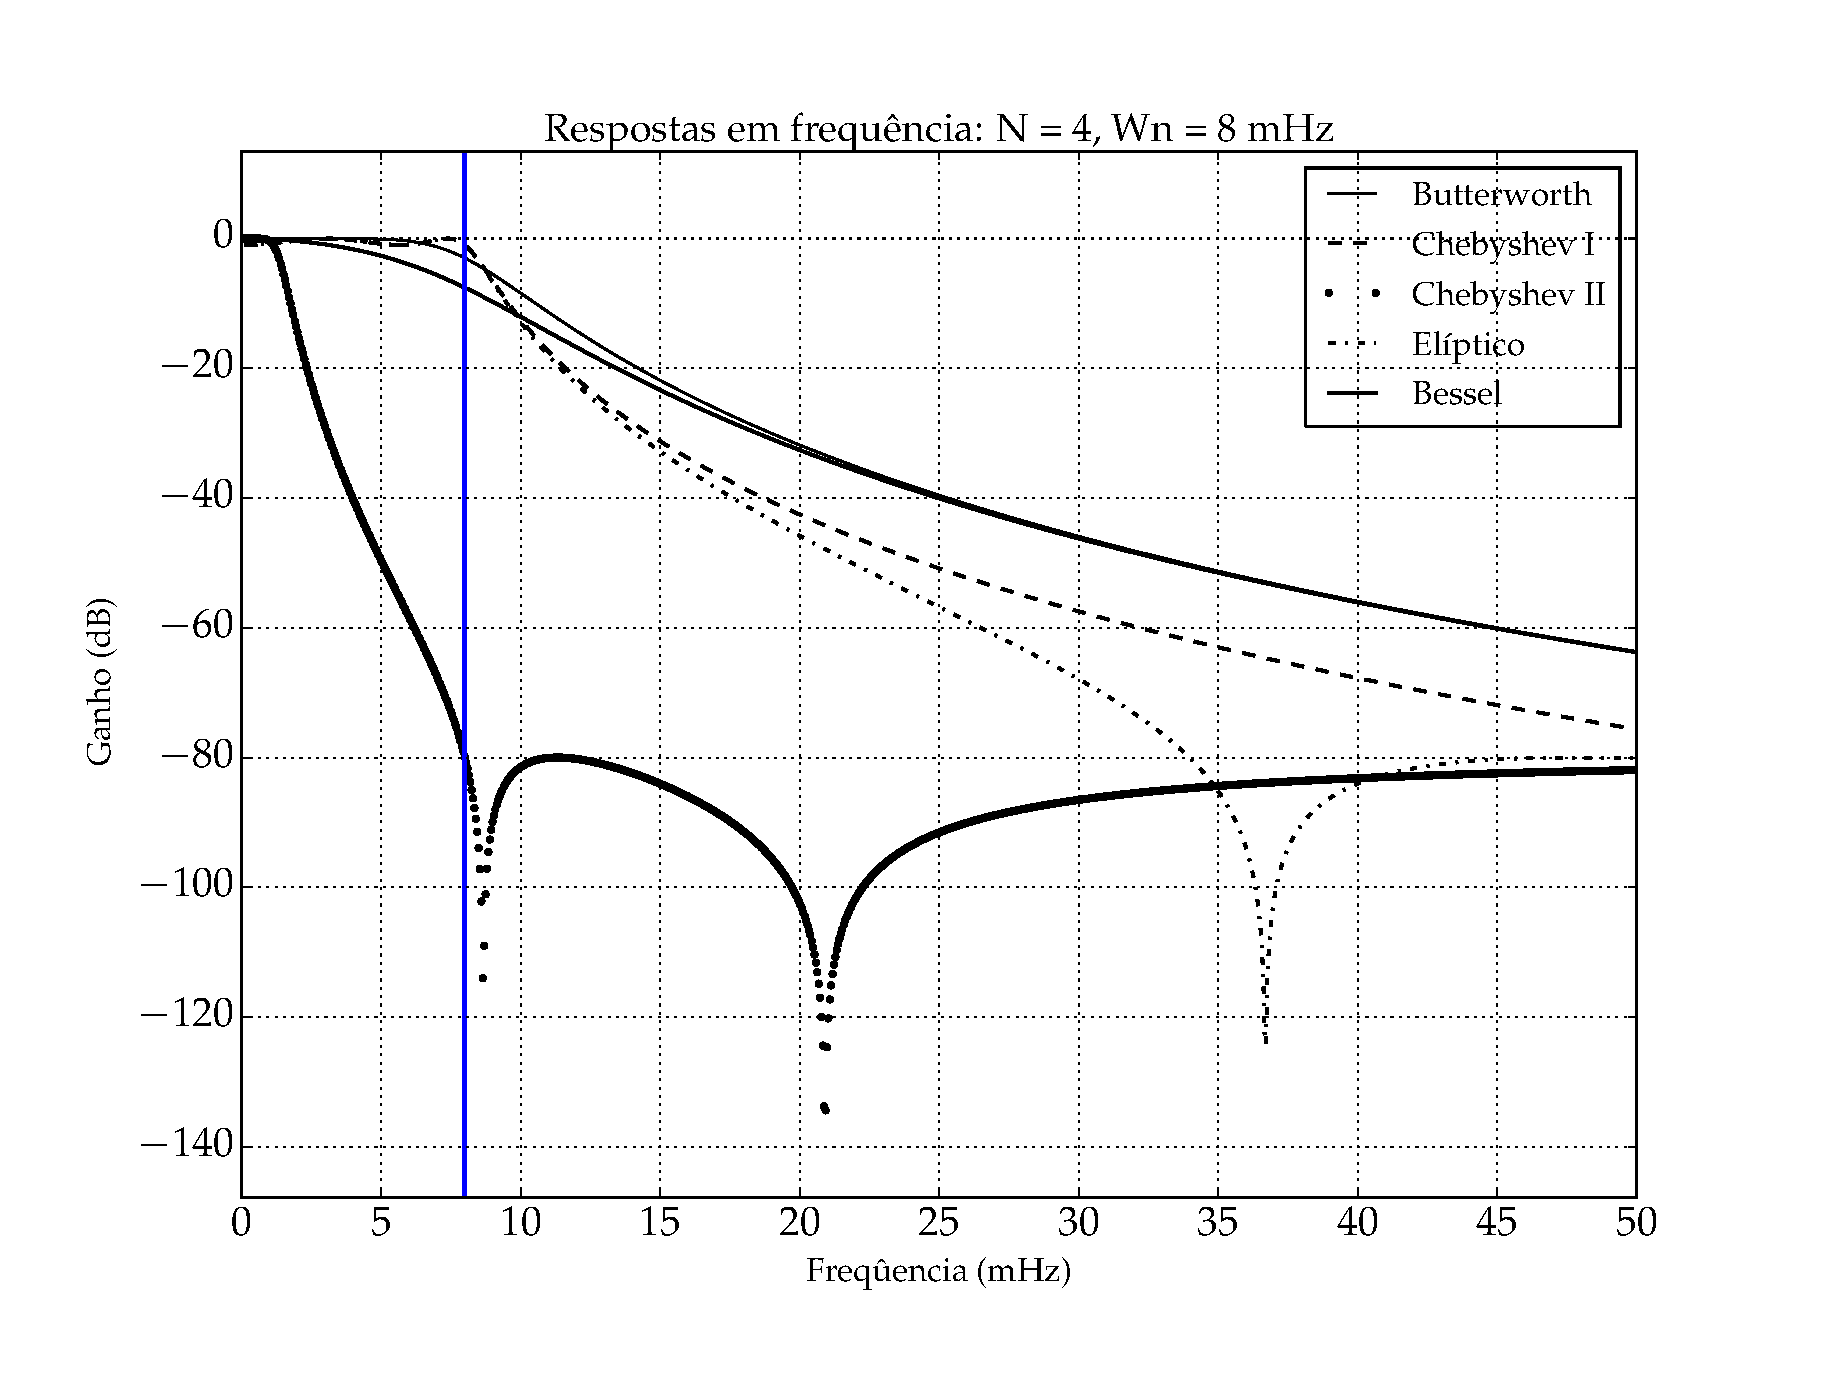
\includegraphics[scale=0.55]{images/plots/lowpass_analog}
  \caption{Resposta em frequência para filtro low-pass analógico. }
  \label{fig:lowpass_analog_response}
\end{figure}


A partir do resultado obtido, é possível verificar aquilo que foi afirmado na fundamentação teórica deste trabalho: filtros Butterworth e Bessel tem uma maior planicidade na banda de passagem, ao passo que os filtros Chebyshev apresentam uma transição mais rápida ao custo de terem maior \textit{ripple}. Constata-se também que, para uma frequência $f \gg f_c$, o filtro de Bessel aproxima o filtro de Butterworth.

\subsection{Projeto Digital: IIR}
Inicialmente, foi tentada uma taxa de amostragem de 1000 Hz, todavia constatou-se que esta era inadequada para a aplicação, pois os coeficientes dos filtros efetivamente tornavam-se zero. Então, estabeleceu-se para este projeto que a taxa de amostragem será de 5 Hz.

\begin{figure}[H]
  \centering
  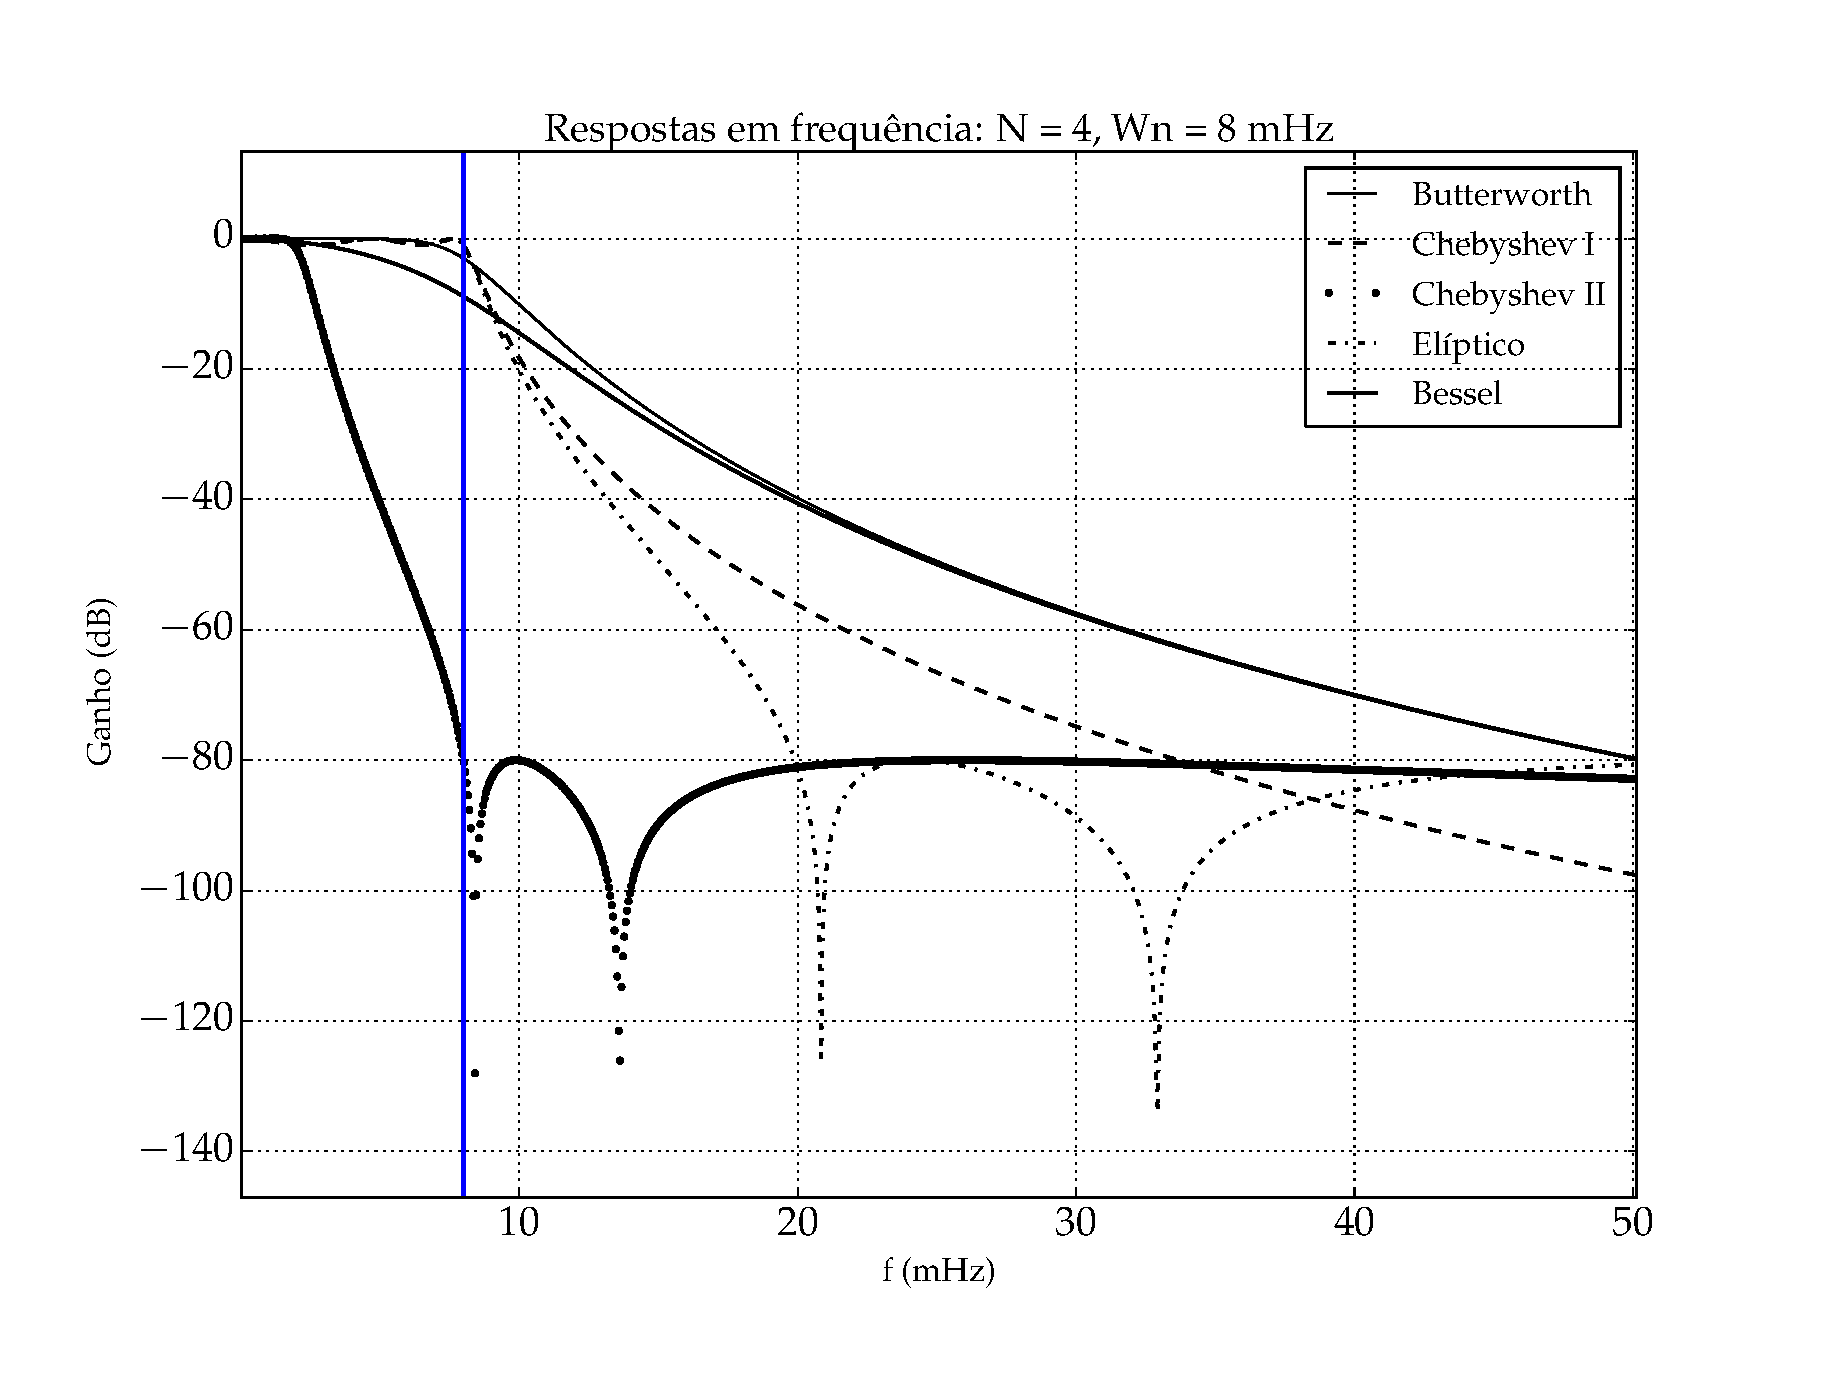
\includegraphics[scale=0.55]{images/plots/lowpass_IIR}
  \caption{Resposta em frequência para filtro low-pass IIR.}
  \label{fig:lowpass_iir_response}
\end{figure}

Constata-se que os resultados obtidos são muito próximos dos resultados do filtro analógico.

\subsection{Projeto Digital: FIR}
Como os filtros FIR são projetados de forma a aproximarem uma resposta em frequência ideal, especificou-se um filtro ideal passa-baixa com frequência de transição de 8 $mHz$; na banda de parada, definiu-se uma atenuação de 80 dB. Obteve-se:

\begin{figure}[H]
  \centering
  \includegraphics[scale=0.45]{images/plots/lowpass_FIR_rectangular_window}
  \caption{Resposta em frequência para filtro low-pass FIR com janela retangular.}
  \label{fig:lowpass_fir_rectang_response}
\end{figure}

\begin{figure}[H]
  \centering
  \includegraphics[scale=0.45]{images/plots/lowpass_FIR_hamming_window}
  \caption{Resposta em frequência para filtro low-pass FIR com janela de Hamming.}
  \label{fig:lowpass_fir_hamming_response}
\end{figure}

Verifica-se que, para ordens muito baixas, o filtro é incapaz de atender os requisitos especificados; já se esta for aumentada, os filtros apresentam maior proximidade daquele especificado, ao custo de maior \textit{ripple} na banda de parada.

A partir dos resultados apresentados nesta seção, pode-se afirmar que filtros digitais IIR são uma ferramenta possível para a filtragem de sinais de baixa frequência, devendo porém a taxa de amostragem ser compatível com a frequência dos sinais a serem processados.

\section{Exemplo de projeto: filtro \textit{notch}}
\label{sec:notch}
Uma aplicação bastante comum do projeto de filtros é o projeto de filtros \textit{notch} para remoção do ruído de 60 Hz da rede elétrica de um sinal. O filtro a ser projetado será um \textit{band-stop} cujas frequências de -3 dB são 59 e 61 Hz. 

Para o projeto dos filtros analógico e IIR definiu-se que o \textit{ripple} máximo aceitável é de 1 dB e que a atenuação na banda de parada será de 80 dB.

\subsection{Projeto Analógico}
Na figura \ref{fig:bandstop_analog_response} apresentam-se as respostas em frequência de um filtro \textit{band-stop} de 5\textsuperscript{a} ordem, nas frequências de corte especificadas anteriormente, para diferentes funções de transferência:

\begin{figure}[H]
  \centering
  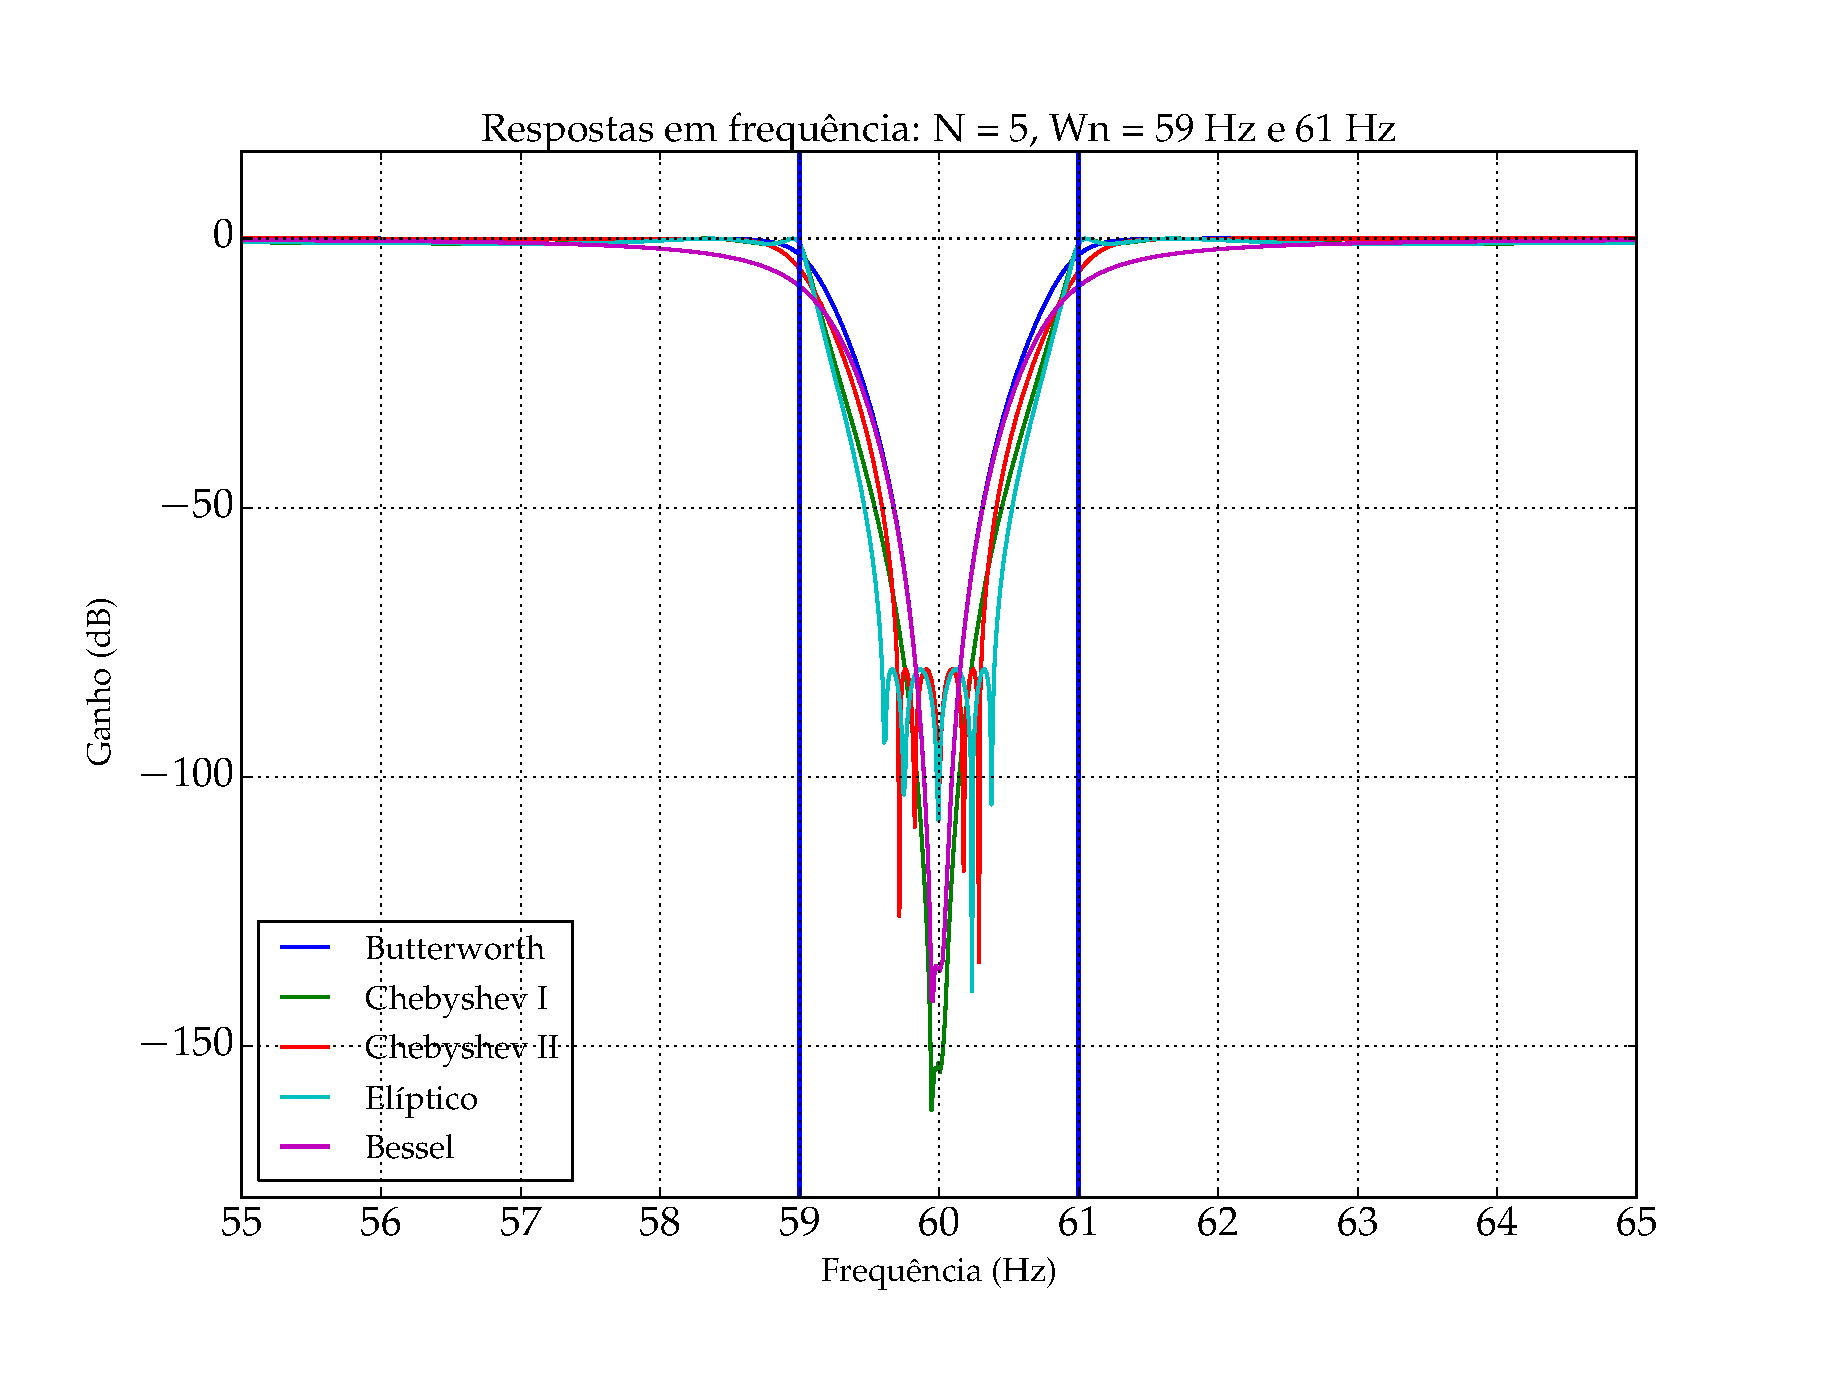
\includegraphics[scale=0.48]{images/plots/bandstop_analog}
  \caption{Resposta em frequência para filtro band-stop analógico.}
  \label{fig:bandstop_analog_response}
\end{figure}

Verifica-se o comportamento descrito na revisão teórica do presente trabalho, sendo que no filtro Chebyshev tipo II, a(s) frequência(s) $\omega_n$ representam os pontos nos quais é atingida a atenuação na banda de parada (ao contrário dos outros filtros, onde elas representam as frequências de $-3$ dB).

\subsection{Projeto Digital: IIR}
Projetou-se um filtro com especificações similares ao do analógico apresentado anteriormente, sendo a frequência de amostragem definida em 1000 Hz. Obteve-se a seguinte resposta em frequência:

\begin{figure}[H]
  \centering
  \includegraphics[scale=0.55]{images/plots/bandstop_IIR}
  \caption{Resposta em frequência para filtro band-stop IIR.}
  \label{fig:bandstop_IIR_response}
\end{figure}

As mesmas conclusões feitas no item anterior para os filtros analógicos podem ser feitas aqui; todavia, constata-se a presença de pequenas e praticamente desprezíveis oscilações devido ao processo de discretização.

\newpage
\subsection{Projeto Digital: FIR}
O projeto deste filtro é especificado em função de ganhos e bandas; dessa forma, define-se:

\begin{itemize}
\item{\textbf{Banda de passagem}}: 0-58 Hz e 61-500 Hz, com ganho de 0 dB;
\item{\textbf{Banda de parada}}: 59-61 Hz, com atenuação de 80 dB.
\end{itemize}

Foram obtidos os seguintes resultados para diferentes números $N$ de \textit{taps}\footnote{Não há uma regra geral para estimar a ordem necessária; desta forma, o processo muitas vezes envolve a simulação com diferentes ordens até atingida a resposta desejada}, quando empregada a função janela retangular:

\begin{figure}[H]
  \centering
  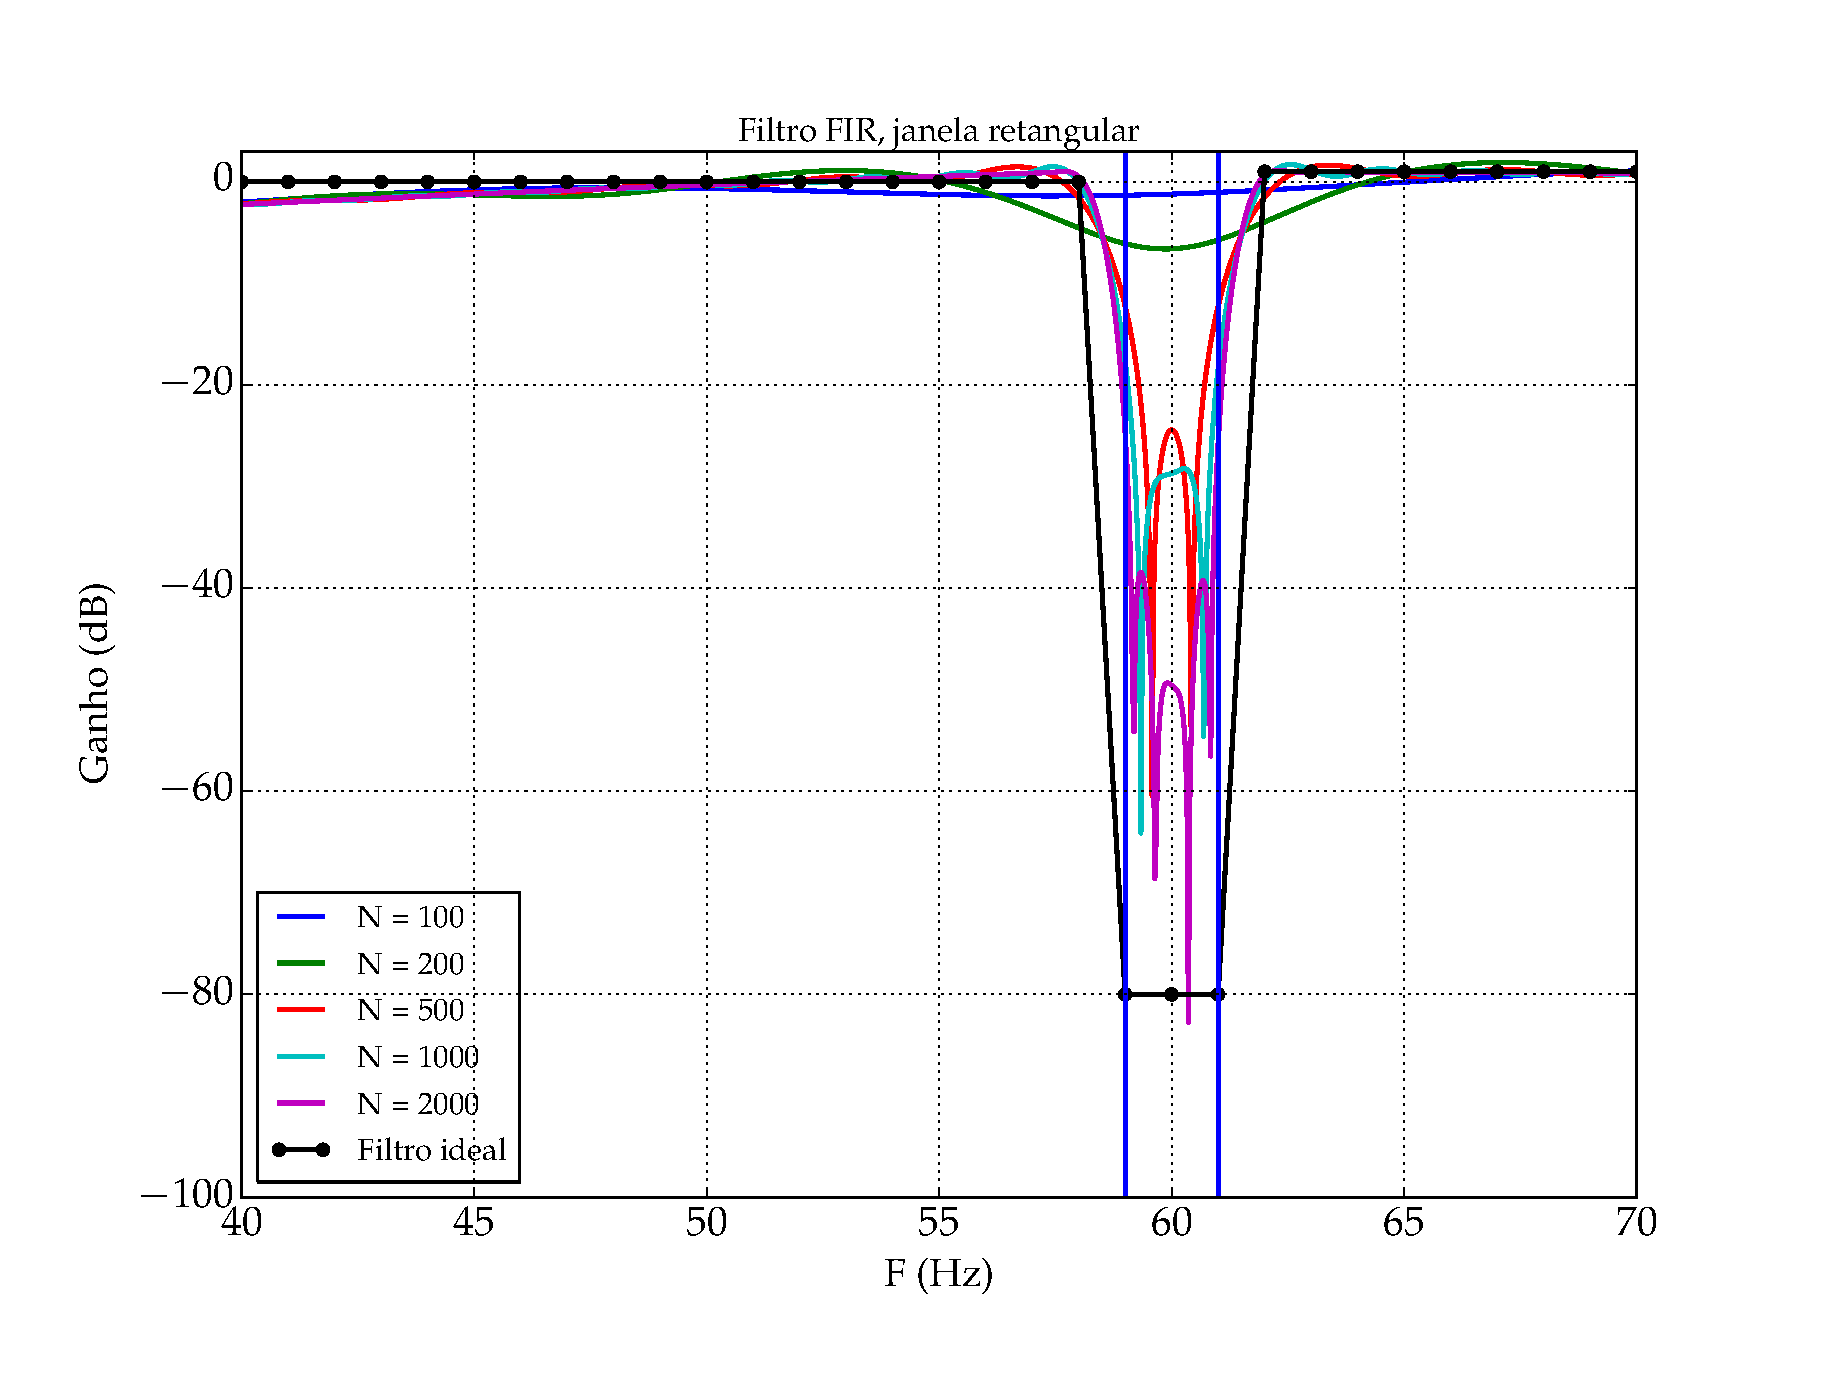
\includegraphics[scale=0.55]{images/plots/bandstop_FIR_rectangular_window}
  \caption{Resposta em frequência para filtro band-stop FIR com a função janela retangular.}
  \label{fig:bandstop_FIR_rectangular}
\end{figure}

\newpage
Quando é empregada a função janela de Hamming, tem-se o seguinte resultado:

\begin{figure}[H]
  \centering
  \includegraphics[scale=0.55]{images/plots/bandstop_FIR_hamming_window}
  \caption{Resposta em frequência para filtro band-stop FIR com a função janela de Hamming.}
  \label{fig:bandstop_FIR_hamming}
\end{figure}

\newpage

Já para a janela triangular, tem-se:

\begin{figure}[H]
  \centering
  \includegraphics[scale=0.55]{images/plots/bandstop_FIR_triang_window}
  \caption{Resposta em frequência para filtro band-stop FIR com a função janela  triangular.}
  \label{fig:bandstop_FIR_triangular}
\end{figure}

De imediato constata-se que, para atingir o mesmo desempenho dos filtros IIR, é necessário um número maior de iterações. Verifica-se que as funções janela de Hamming e triangular não tem o \textit{ripple} na banda de parada, ao custo de apresentarem uma menor atenuação - e também pode ser visto que a função janela triangular é inadequada para a aplicação proposta. A função janela retangular, também, atinge um resultado mais próximo dos filtros IIR elíptico e Chebyshev tipo II.

\newpage

Para o filtro \textit{equirripple} sintetizado pelo algoritmo de Parks-McClellan, é obtido: 

\begin{figure}[H]
  \centering
  \includegraphics[scale=0.55]{images/plots/bandstop_fir_pm}
  \caption{Resposta em frequência para filtro band-stop FIR projetado pelo algoritmo de Parks-McClellan.}
  \label{fig:bandstop_FIR_pm}
\end{figure}

Para o filtro implementado por esse algoritmo, tem-se uma imposição do algoritmo que requer que filtros \textit{bandstop} tenham ordem ímpar, caso contrário os objetivos não são atingidos.

Pode-se verificar que esta família de filtros apresenta o \textit{ripple} igual para todas as frequências na banda de passagem,  sendo que este é inversamente proporcional à ordem do filtro ao custo de oscilações na banda de parada.

\newpage
\section{Exemplo de projeto: filtro passa-banda}
\label{sec:bandpass}
Em aplicações de áudio e de telefonia é bastante comum a necessidade de filtros para permitir a passagem da voz humana, na faixa de 300 a 4000 Hz. Para este projeto tem-se as seguintes especificações:

\begin{itemize}
\item \textbf{Bandas de parada}: 100-300 Hz e 4000-6000 Hz.
\item \textbf{Banda de passagem}: 300 a 4000 Hz
\item \textbf{Ripple na banda de passagem}: 3 dB
\item \textbf{Atenuação na banda de parada}: 80 dB
\end{itemize}

e devem-se determinar ordem e frequências críticas que as satisfaçam.

\subsection{Projeto Analógico}

\begin{figure}[H]
  \centering
  \includegraphics[scale=0.55]{images/plots/bandpass_analog}
  \caption{Resposta em frequência para filtro band-pass analógico.}
  \label{fig:bandpass_analog}
\end{figure}

A partir desses resultados, os \textit{trade-offs} entre os diferentes tipos de filtros ficam claros. Verifica-se que o filtro de Butterworth, embora não apresente \textit{ripple}, precisa de maior ordem para atingir resultados similares aos outros filtros; já o filtro de Bessel demonstrou-se insuficiente para atingir a especificação solicitada. O filtro elíptico consegue fornecer, para uma menor ordem, resultados bastante similares às outras topologias.

Um dos problemas já citados anteriormente e que foi constatado nesse exemplo de projeto foram instabilidades numéricas: inicialmente foi tentado o projeto com uma especificação de banda de parada de 4000 a 5000 Hz, porém os algoritmos falhavam ao calcular a resposta em frequência. O MATLAB tenta contornar esse problema calculando o filtro em seções de segunda ordem (\textit{second order sections}), as quais não foram implementadas em Python, ficando em aberto a ideia de sua implementação.

\subsection{Projeto Digital: IIR}
Para este projeto, foi estabelecida uma taxa de amostragem de 20 KHz.

\begin{figure}[H]
  \centering
  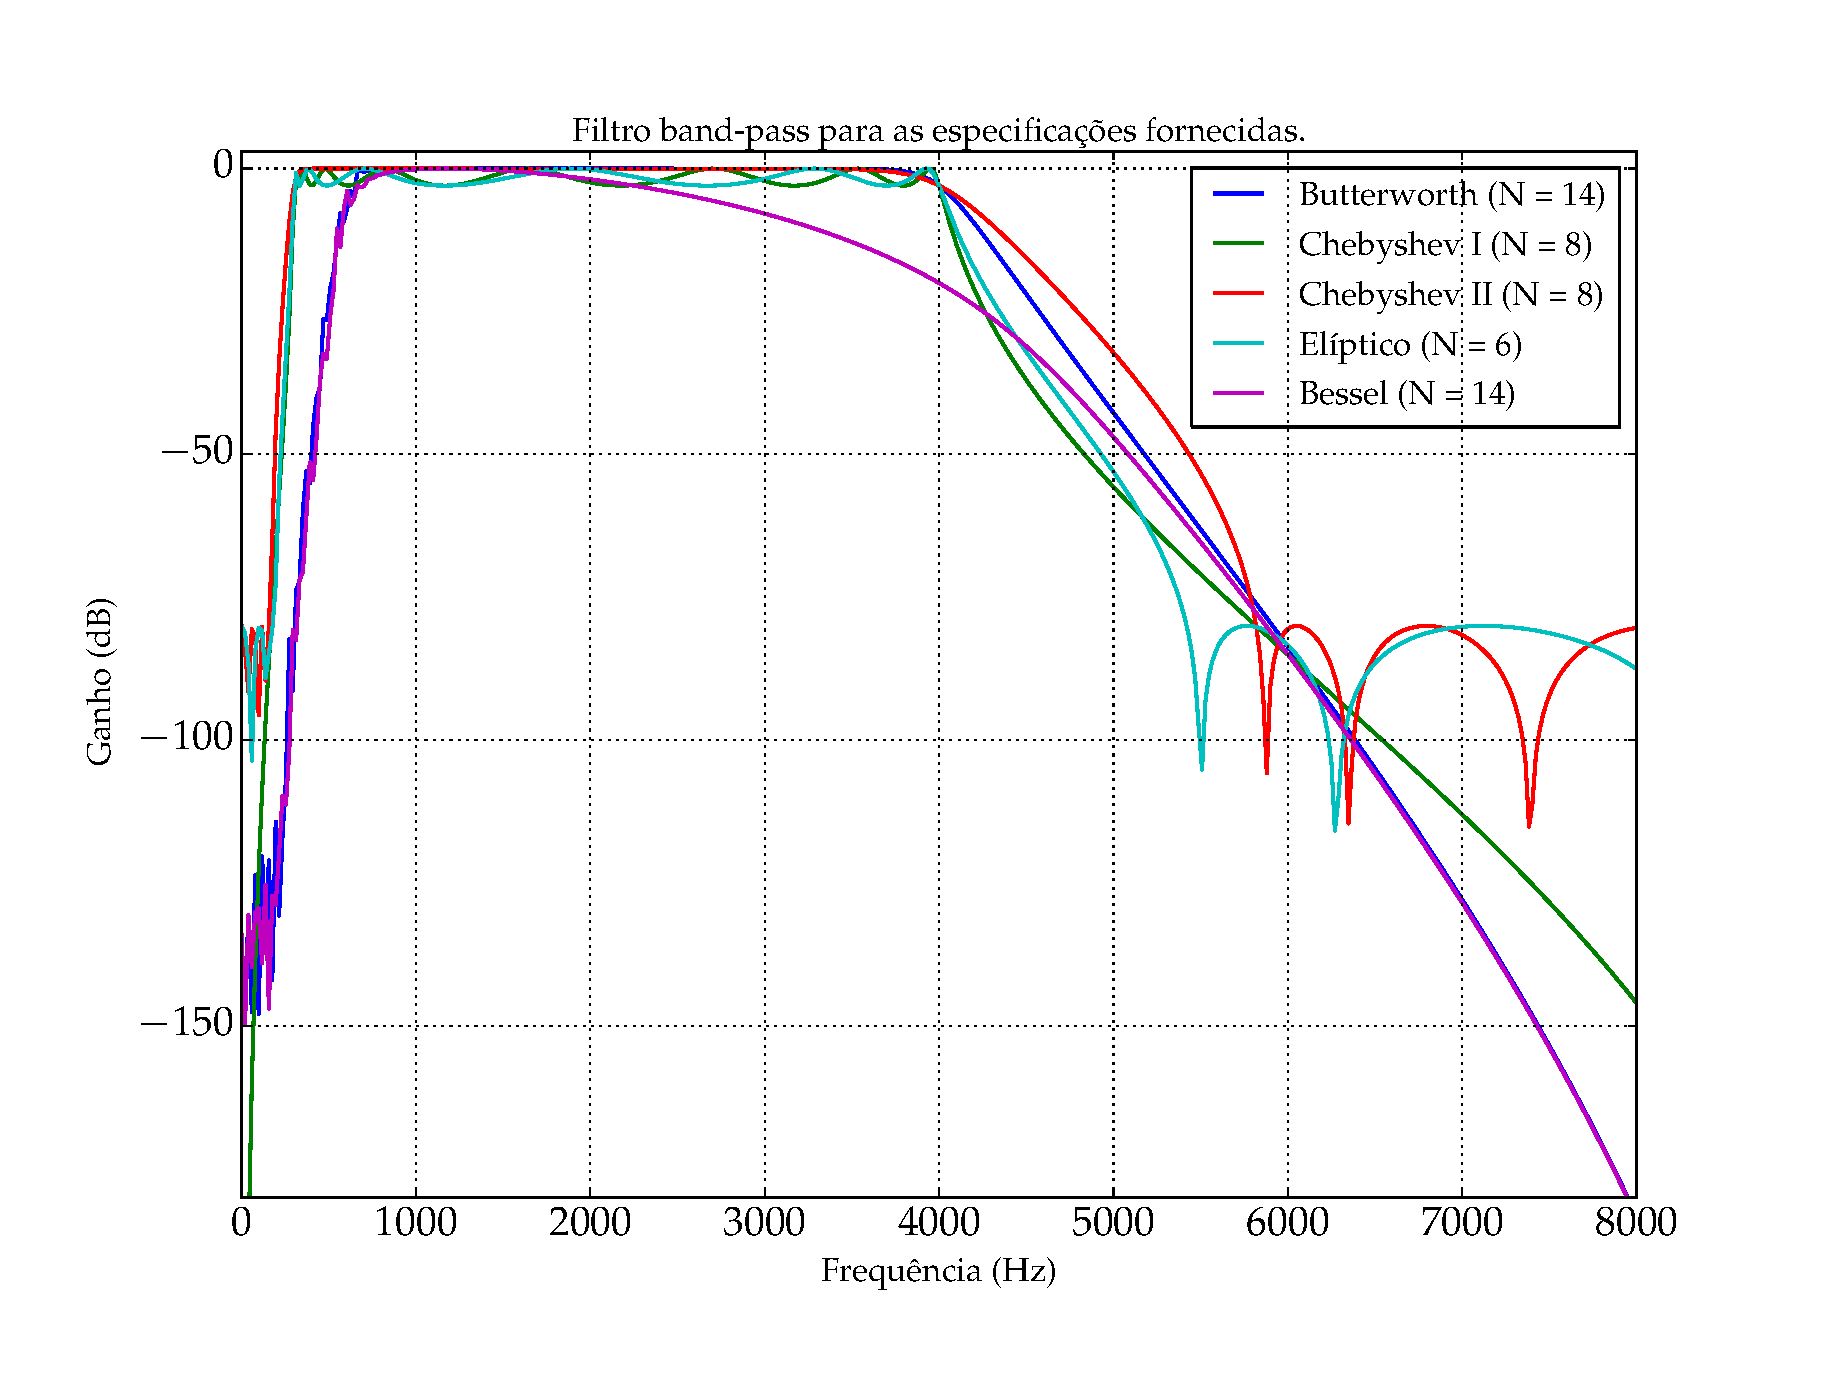
\includegraphics[scale=0.5]{images/plots/bandpass_IIR}
  \caption{Resposta em frequência para filtro band-pass IIR.}
  \label{fig:bandpass_IIR}
\end{figure}

Os resultados de ambos projetos são bem similares, valendo as mesmas conclusões que foram feitas para o projeto analógico.

\subsection{Projeto Digital: FIR}

Foi especificado um filtro ideal, com 0 dB de ganho na faixa de 300 a 4000 Hz e -80 dB fora dela, tendo-se obtido: 

\begin{figure}[H]
  \centering
  \includegraphics[scale=0.55]{images/plots/bandpass_FIR_rectangular_window}
  \caption{Resposta em frequência para filtro band-pass FIR com a função janela retangular.}
  \label{fig:bandpass_FIR_rectangular}
\end{figure}

\begin{figure}[H]
  \centering
  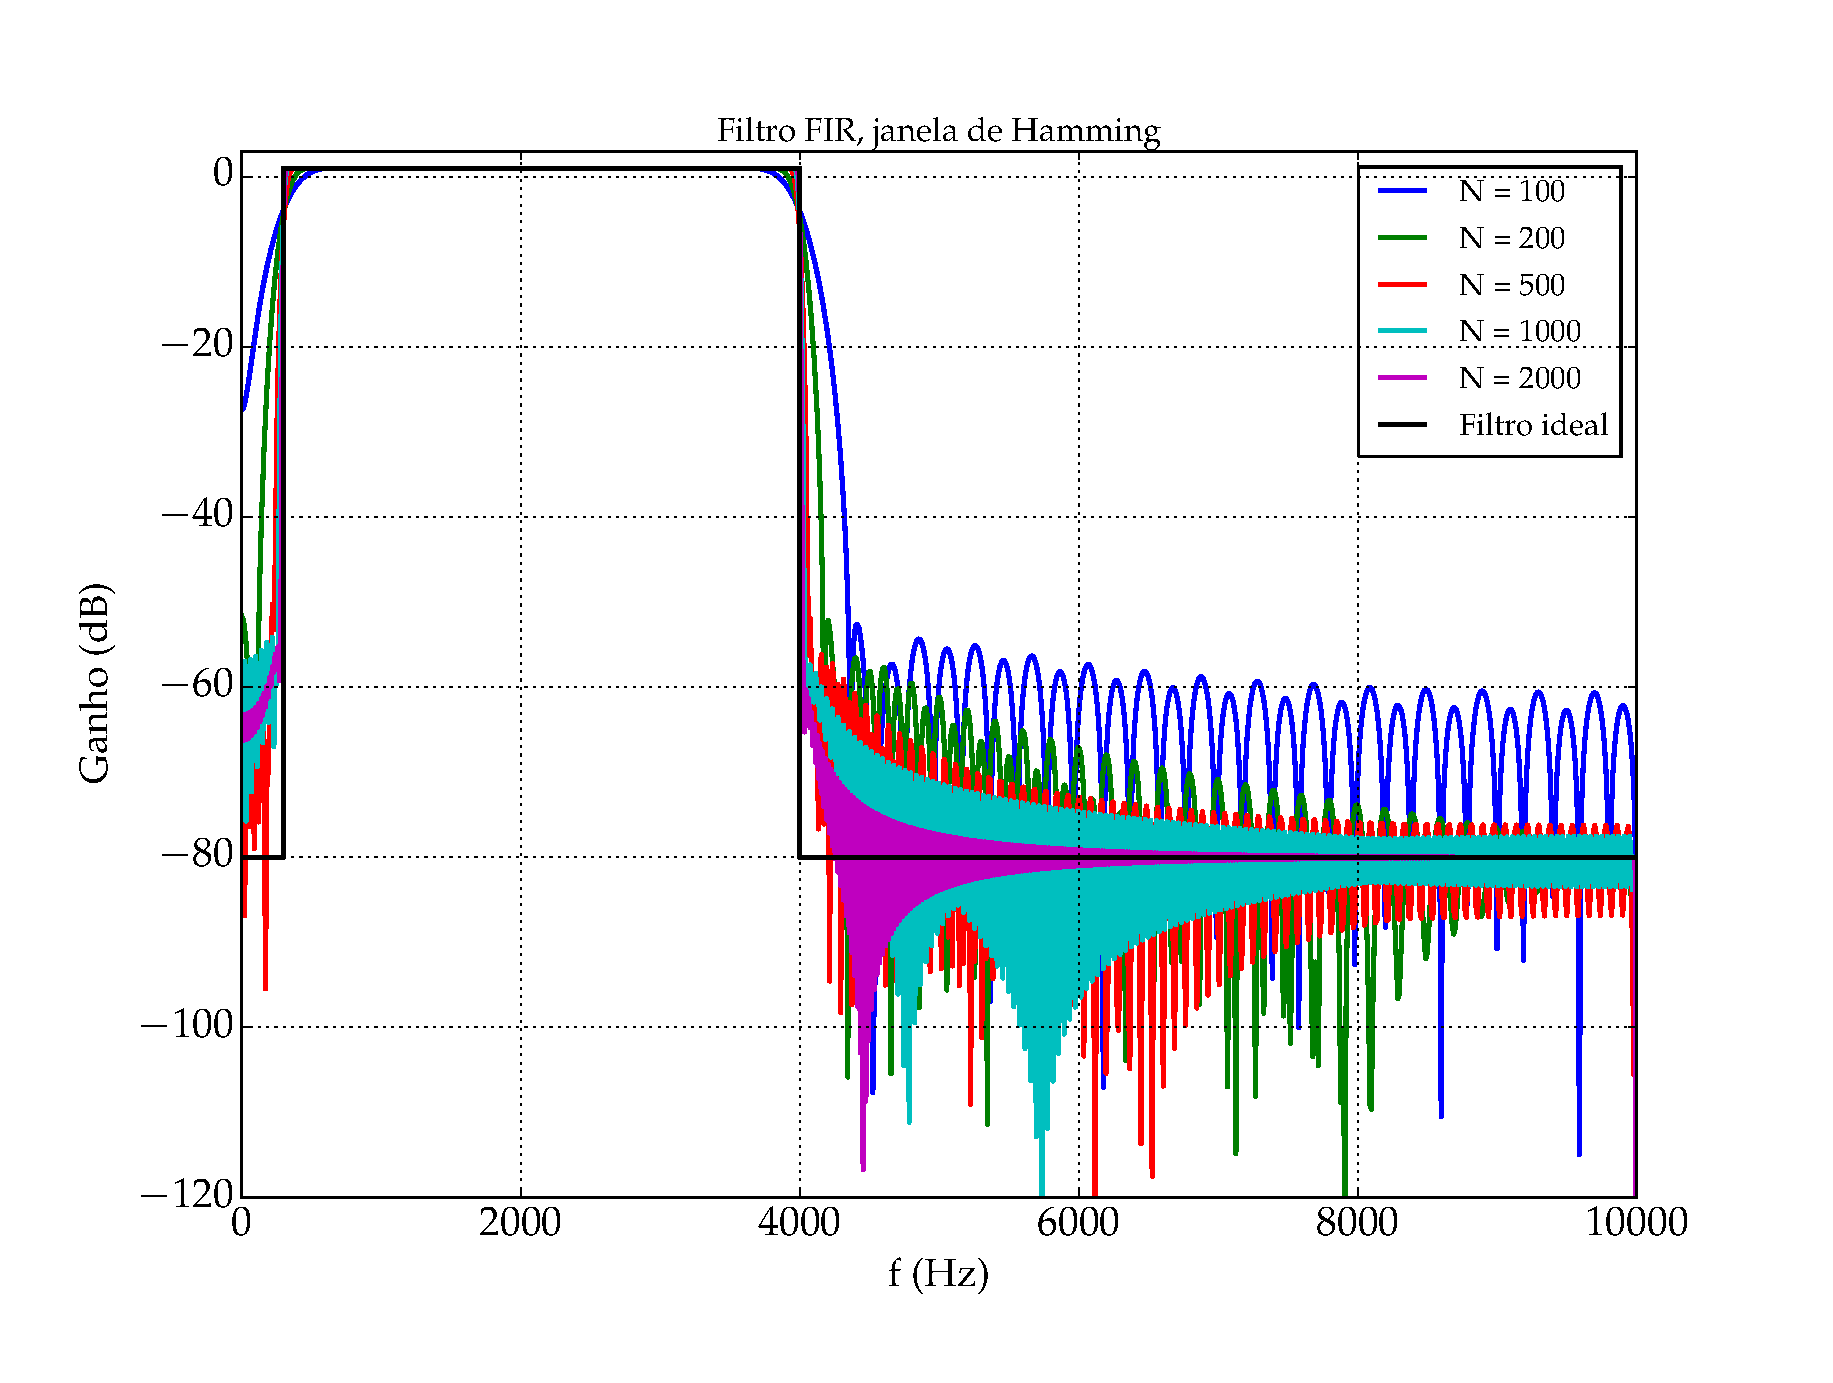
\includegraphics[scale=0.55]{images/plots/bandpass_FIR_hamming_window}
  \caption{Resposta em frequência para filtro band-pass FIR com a função janela de Hamming.}
  \label{fig:bandpass_FIR_hamming}
\end{figure}

\begin{figure}[H]
  \centering
  \includegraphics[scale=0.55]{images/plots/bandpass_FIR_triang_window}
  \caption{Resposta em frequência para filtro band-pass FIR com a função janela triangular.}
  \label{fig:bandpass_FIR_triangular}
\end{figure}

É interessante notar que a implementação FIR para esse filtro permite obter uma resposta bem próxima da ideal. Com a função janela de Hamming e a retangular, temos oscilações na banda de parada, ao passo que, empregando-se a janela triangular, estas não acontecem ao custo de uma transição menos ágil.

A partir dos resultados obtidos para os três projetos, os quais confirmam aquilo que foi afirmado na revisão teórica, verifica-se o funcionamento adequado da ferramenta para aquilo que foi proposto no início deste trabalho.

\newpage

\section{Tempo de Processamento}
Como os filtros analógicos e IIR, conforme observado no desenvolvimento deste trabalho, são implementados por meio da aplicação direta de fórmulas, seu tempo de processamento é desprezível e não será abordado. 

Determinam-se os seguintes tempos de processamento para o projeto de filtros FIR, quando executado para um filtro simples em um computador com CPU Intel Core i7 rodando a 2.2 GHz, com 6 GB de RAM e rodando o Linux Ubuntu 15.04 com Python 3.4.3:

% Tive que converter o EPS para PDF, senão o ShareLaTeX dava algum bug que corrompia o arquivo. 
\begin{figure}[H]
  \centering
  \includegraphics[scale=0.5]{images/plots/fir_benchmark}
 \caption{Tempo de processamento necessário para o projeto de um filtro FIR com N \textit{taps}, pelo método do janelamento. Para cada N o algoritmo foi executado 1000 vezes.}
 \label{fig:fir_benchmark}
\end{figure}

\newpage
Para comparação, um filtro similar foi projetado empregando-se o \textit{MATLAB} versão R2013a no mesmo computador, tendo sido obtido o seguinte resultado:

\begin{figure}[H]
  \centering
  \includegraphics[scale=0.5]{images/plots/fir_comparison}
 \caption{Comparação do tempo tempo de processamento necessário entre Python e MATLAB para o projeto, com as mesmas condições do item \ref{fig:fir_benchmark}.}
 \label{fig:fir_comparison}
\end{figure}


A partir do gráfico \ref{fig:fir_benchmark}, podemos afirmar que o tempo de processamento gasto cresce de forma aproximadamente exponencial com o número de \textit{taps} desejado. Já em \ref{fig:fir_comparison}, verifica-se que o MATLAB apresenta desempenho idêntico ou melhor ao Python; presume-se que esse fenômeno ocorre devido ao fato do MATLAB ter diversas otimizações em suas bibliotecas, porém não é possível confirmar essa hipótese visto que o MATLAB é um \textit{software} de código fechado.

\section{Comparação com Ferramentas já Existentes}
\label{sec:tool_comparison}
Para guiar o desenvolvimento das funcionalidades da ferramenta elaborada no presente trabalho, realizou-se um estudo com algumas das diversas ferramentas já existentes no mercado. 

Para o caso dos filtros analógicos, elas fornecem o circuito projetado; já para os filtros digitais, os coeficientes são fornecidos.  

Também nota-se que o fluxo de trabalho em todas elas é similar: a partir das especificações desejadas, determinam-se funções de transferência ou circuitos que as implementam. 

\subsection{Analog Filter Wizard (Analog Devices)}
Esta ferramenta gratuita, disponível em \cite{analog} é voltada ao projeto de filtros analógicos e implementa os filtros de Bessel, Butterworth e Chebyshev tipo I, com ordens limitadas a 10, permitindo ao usuário decidir entre menos estágios e menor tempo de acomodação.

Uma função interessante dessa ferramenta é permitir algumas otimizações para o circuito (por exemplo, menor consumo de energia ou menor ruído) e realizar a análise das tolerâncias dos componentes: pode-se verificar como o circuito irá se comportar perante a variabilidade dos resistores e capacitores empregados.

\begin{figure}[H] 
\centering \includegraphics[scale=0.33]{images/screens/afd_in}
\centering \includegraphics[scale=0.33]{images/screens/afd_out}
\caption{Exemplo da interface do \textit{Analog Filter Wizard}: entrada de dados e resultados.} 
\label{fig:afw_example} 
\end{figure}

\subsection{FilterPro (Texas Instruments)}
Esta ferramenta disponível em \cite{ti_filter} roda no \textit{browser} (é escrita em \textit{Flash}) e permite diversas otimizações no circuito projetado (reduzir o número de componentes ou o custo desses, maximizar a atenuação na banda de parada, minimizar o \textit{ripple} na banda de passagem). 

Assim como o \textit{Analog Filter Wizard}, os circuitos são implementados utilizando-se as topologia \textit{multiple feedback} ou \textit{Sallen-Key.}

\begin{figure}[H] 
\centering \includegraphics[scale=0.33]{images/screens/fp_example} \caption{Exemplo da interface do \textit{FilterPro}.} 
\label{fig:fp_example} 
\end{figure}

\subsection{DSP System Toolbox (MATLAB)}

Este pacote de ferramentas disponível para o MATLAB é voltado ao projeto de filtros digitais, sendo o mais completo dentre as ferramentas analisadas e cobrindo tanto filtros FIR quanto IIR - para os quais estão implementadas diversos algoritmos de cálculo (método da janela, Parks-McClellan, mínimos quadrados etc...).

Pode ser operado em linha de comando e por meio de interface gráfica, sendo que seu funcionamento e a funcionalidade são similares em ambos; enquanto a interface gráfica permite o projeto interativo, a linha de comando permite o emprego dos filtros projetados em rotinas mais complexas para processamento de sinais.

Uma das suas funcionalidades mais relevantes, considerado que filtros digitais são amplamente empregados em sistemas embarcados, é a sua capacidade de gerar código-fonte em C e em VHDL para uso em CPUs.

\begin{figure}[H] 
\centering \includegraphics[scale=0.5]{images/screens/fdatool_example} \caption{Exemplo da interface do \textit{Filter Design and Analysis tool}.} 
\label{fig:fda_example} 
\end{figure}

Comparado às ferramentas existentes, a ferramenta apresentada no presente trabalho tem como principal vantagem não ter limitações de ordem do filtro projetado (excetuando-se, conforme descrito no desenvolvimento, o filtro de Bessel que é implementado por meio de tabelas que vão apenas até a 25\textsuperscript{a} ordem).

Outro importante aspecto é que as ferramentas acima descritas são \textit{caixas pretas} de código fechado. Embora, para o usuário, isso muitas vezes não seja um fator limitante ou incômodo, sua funcionalidade está restrita àquela que os desenvolvedores da ferramenta implementaram: há pouca ou nenhuma possibilidade de expansão ou de integração em um algoritmo ou aplicação mais complexa.

A ferramenta desenvolvida aqui, entretanto, tem seu código aberto (\textit{open source}) e também baseada em bibliotecas abertamente disponíveis. Dessa forma, além da vantagem imediata do custo \footnote{Uma licença do MATLAB com as bibliotecas de processamento de sinais e de DSP custa em média US\$ 5 mil}, ela pode ser modificada e expandida pelos seus usuários, que podem adicionar novas funcionalidades e estudar seu código-fonte para entender o funcionamento.

Todavia, não foram implementadas todas funcionalidades existentes nas ferramentas apresentadas: as ferramentas para projeto de filtros analógicos não realizam a síntese de circuitos, já para projeto digital não é gerado código para implementação em uma CPU. No item \ref{sec:improvements} descrevem-se melhorias que podem ser realizadas com o objetivo de dar continuidade a este trabalho e permitir que ele atinja o patamar das ferramentas existentes.
\chapter{Conclusão}

Neste trabalho, demonstrou-se com sucesso o desenvolvimento de uma ferramenta computacional para a síntese de filtros analógicos e digitais; sua vantagem imediata perante as ferramentas já existentes é ser gratuita e de código aberto, em contraste com as existentes, \textit{caixas pretas} que permitem pouca ou nenhuma modificação ou estudo e, em alguns casos, possuem licenças bastante caras.

O usuário pode estudar o código-fonte da ferramenta e das bibliotecas empregadas e entender o seu funcionamento, os algoritmos empregados e as decisões tomadas durante o desenvolvimento. Isto é facilitado pela linguagem \textit{Python}, cuja sintaxe é bastante clara e acessível mesmo para usuários com pouco conhecimento de programação.

Soma-se a essas vantagens a possibilidade de desenvolvimento de novas funcionalidades, que podem ser contribuídas por qualquer desenvolvedor interessado em dar continuidade ao trabalho: basta que ele desenvolva e teste a função desejada e submeta seu código para o autor do \textit{software}, que se encarregará de incorporá-la ao programa. Da mesma forma, eventuais melhorias ou correções de \textit{bugs} que sejam feitas nas bibliotecas empregadas neste projeto podem ser contribuídas aos seus projetos de origem.

Por fim, os algoritmos e códigos desenvolvidos neste trabalho podem ser aproveitados em outros projetos, assim possibilitando o desenvolvimento de novas ferramentas baseadas no que foi apresentado aqui. 

O código-fonte do \textit{software} desenvolvido aqui, juntamente com outras rotinas (por exemplo, \textit{scripts} usados para teste e para geração dos gráficos) está disponível na plataforma GitHub, no endereço \url{https://github.com/renanbirck/pyfilter}, sob licença de \textit{software} livre, para permitir que seu desenvolvimento seja continuado.

\newpage
\section{Futuras melhorias}
\label{sec:improvements}
Para a continuidade deste trabalho com o objetivo de torná-lo uma ferramenta completa para o projeto de filtros, possíveis melhorias incluem, mas não estão limitadas, às seguintes:

\subsection{Análise de Estabilidade}
Como afirmado na fundamentação teórica, filtros analógicos e filtros digitais IIR, por possuírem \textit{feedback}, estão sujeitos à instabilidade, principalmente quando são empregados em sistemas de controle (aplicação comum para a filtragem de sinais).

Dessa forma, torna-se desejável que a ferramenta seja capaz de realizar o estudo da estabilidade do filtro projetado. 

\subsection{Análise de Sensitividade}
Circuitos analógicos reais são implementados com componentes não-ideais, ao passo que os projetos de filtros são realizados presumindo-se que os dispositivos empregados são ideais. Como consequência, existe o risco do circuito implementado não corresponder àquilo que foi projetado. 

Analisar a saída do circuito perante não-linearidades e variações dos componentes empregados nele torna-se uma funcionalidade necessária, a qual pode ser implementada interfaceando-se a ferramenta com um simulador de circuitos que será encarregado dos cálculos. 

\subsection{Aperfeiçoamentos na Interface Gráfica}
Tornar a interface gráfica da ferramenta mais simples de usar e realizar melhorias no quesito de intuitividade e interação com o usuário; verificar a viabilidade do uso de outras bibliotecas de interface gráfica (por exemplo, a IUP - Portable User Interface \cite{iup}, que também é de código aberto e é voltada a aplicações científicas).

\subsection{Emprego de Algoritmos de Otimização}
Como foi visto, é possível descrever o projeto de filtros como um problema de otimização matemática: deseja-se encontrar parâmetros para um sistema LTI que melhor aproximem uma resposta não-causal. 

Esta estratégia, cuja viabilidade já foi demonstrada com sucesso na literatura (é a forma com que opera o algoritmo de Parks-McClellan; outros autores empregam diferentes técnicas de otimização, por exemplo, em \cite{barros} são empregados algoritmos genéticos), torna-se particularmente desejável quando são conhecidas as características do filtro desejado, porém não se conhece qual a ordem e quais as frequências que atendem essa especificação.

\subsection{Geração de Código}
Filtros digitais geralmente são implementados em CPUs programadas na linguagem C ou Assembly, ou em FPGAs programados em VHDL. Torna-se, então, desejável que a ferramenta seja capaz de produzir código nessas linguagens.

Isso levanta as considerações de implementação descritas na revisão teórica deste trabalho, como os tipos de dados das variáveis e questões relacionadas à precisão numérica, além das estruturas de implementação (por exemplo, formas diretas I e II) que deverão ser empregadas para evitar polinômios de alta ordem e suas instabilidades numéricas.

\subsection{Interface em Linha de Comando e Biblioteca de Funções}
Embora a interface gráfica seja uma ferramenta prática para o usuário da ferramenta, ela limita o usuário às funcionalidades que o seu desenvolvedor julga úteis. 

Dessa forma, é desejável que as funções para projeto possam ser empregadas diretamente em outros códigos, inclusive como parte de um sistema maior.

Uma separação rígida entre interface e algoritmo também melhora a qualidade do código de ambos, pois cada parte pode ser testada, melhorada e modificada isoladamente, reduzindo-se o risco de afetar funcionalidades já existentes.

\subsection{Realização de Análises}
É desejável que o usuário possa analisar o filtro projetado quanto a resposta no tempo (por exemplo, verificar como ele se comporta com uma resposta ao impulso ou ao degrau unitário) e no plano complexo. 

Isto permite que o usuário julgue o filtro obtido quanto à estabilidade e fornece uma ferramenta intuitiva para o entendimento de como a posição dos polos e zeros do filtro afeta as características dele.

\subsection{Síntese de Circuitos}
Filtros analógicos podem ser implementados com as topologias vistas na introdução; para colocar a ferramenta apresentada neste trabalho no mesmo patamar daquelas descritas no item \ref{sec:tool_comparison}, pode-se considerar que esta funcionalidade é essencial, devendo ser uma das prioridades de desenvolvimento.

Juntamente com um simulador de circuitos, torna-se possível analisar o comportamento dos filtros sob condições não-ideais tais como o uso de \textit{op-amps} reais ou a variabilidade dos componentes.

\chapter{Referências}

Python 3.4.3 Documentation. Disponível em \url{https://docs.python.org/3/}. Acesso em 03 mar. 2015.


\setlength{\baselineskip}{\baselineskip}

%%=============================================================================
%% Referências
%%=============================================================================
%\bibliographystyle{abnt}
%\bibliography{referencias/referencias}



%IMPORTANTE: Se precisar usar alguma seção ou subseção dentro dos apêndices ou
%anexos, utilizar o comando \tocless para não adicionar no Sumário
%Exemplos: 
% \tocless\section{Histórico}
%%=============================================================================
%% Apêndices
%%=============================================================================
%\appendix
%
\chapter{Título do apêndice}
Este é o apêndice A

%IMPORTANTE: Se precisar usar alguma seção ou subseção dentro dos apêndices ou
%anexos, utilizar o comando \tocless para não adicionar no Sumário
%Exemplos: 
% \tocless\section{Histórico}
% \tocless\subsection{Detalhes}
\tocless\section{teste}
Este é um teste de seção dentro do apêndice


%
\chapter{Título do apêndice Ex}
Esta é o apêndice B




\end{document}
